\documentclass[8pt,aspectratio=1610]{beamer}
\usepackage[utf8]{inputenc}
\usepackage{booktabs}
\usepackage{array}
\usepackage{graphicx}
\usepackage{xcolor}
\usepackage{tikz}
\usetikzlibrary{positioning,arrows.meta,decorations.pathreplacing,calc,shadows}
\usepackage{pgfplots}
\pgfplotsset{compat=1.18}
\usepackage{amsmath}
\usepackage{amssymb}
\usepackage{amsfonts}
\usepackage{algorithm}
\usepackage{algorithmic}

\usetheme{metropolis}
\usecolortheme{wolverine}
\metroset{progressbar=frametitle,block=fill}
\setbeamertemplate{navigation symbols}{}

% Define custom colors complementing the Wolverine theme
\definecolor{maizelight}{RGB}{255, 203, 5}      % Light maize for examples
\definecolor{maizedark}{RGB}{255, 167, 0}       % Darker maize for emphasis
\definecolor{bluelight}{RGB}{0, 39, 76}         % Deep blue for blocks
\definecolor{tealaccent}{RGB}{0, 128, 128}      % Teal for variety
\definecolor{orangeaccent}{RGB}{255, 138, 51}   % Orange complement

% Parameter estimation specific colors
\definecolor{momcolor}{RGB}{33, 150, 243}       % Blue for Method of Moments
\definecolor{mlecolor}{RGB}{255, 193, 7}        % Amber for MLE
\definecolor{paramcolor}{RGB}{76, 175, 80}      % Green for parameters
\definecolor{estimatecolor}{RGB}{156, 39, 176}  % Purple for estimates

% Customize block colors
\setbeamercolor{block title}{bg=bluelight,fg=white}
\setbeamercolor{block body}{bg=bluelight!10,fg=black}

% Example blocks in complementary maize
\setbeamercolor{block title example}{bg=maizelight,fg=black}
\setbeamercolor{block body example}{bg=maizelight!15,fg=black}

% Alert blocks in orange accent
\setbeamercolor{block title alerted}{bg=orangeaccent,fg=white}
\setbeamercolor{block body alerted}{bg=orangeaccent!15,fg=black}

% Create custom colored blocks for variety
\newenvironment<>{techblock}[1]{%
  \setbeamercolor{block title}{bg=tealaccent,fg=white}%
  \setbeamercolor{block body}{bg=tealaccent!10,fg=black}%
  \begin{block}#2{#1}}{\end{block}}

\newenvironment<>{momblock}[1]{%
  \setbeamercolor{block title}{bg=momcolor,fg=white}%
  \setbeamercolor{block body}{bg=momcolor!10,fg=black}%
  \begin{block}#2{#1}}{\end{block}}

\newenvironment<>{mleblock}[1]{%
  \setbeamercolor{block title}{bg=mlecolor,fg=black}%
  \setbeamercolor{block body}{bg=mlecolor!15,fg=black}%
  \begin{block}#2{#1}}{\end{block}}

\title{Parameter Estimation}
\subtitle{Method of Moments \& Maximum Likelihood Estimation}
\author{CMSC 173: Machine Learning}
\date{\today}

\begin{document}

\frame{\titlepage}

\begin{frame}{Course Outline}
\setlength{\itemsep}{2pt}
\begin{itemize}
\item \textbf{Introduction} - What is parameter estimation?
\item \textbf{Statistical Foundations} - Key concepts and notation
\item \textbf{Method of Moments} - Classical parameter estimation
\item \textbf{Maximum Likelihood Estimation} - Optimal parameter estimation
\item \textbf{Comparison} - When to use which method
\item \textbf{Applications} - Real-world examples
\item \textbf{Advanced Topics} - Extensions and modern approaches
\item \textbf{Best Practices} - Common pitfalls and guidelines
\end{itemize}
\end{frame}

% SECTION 1: INTRODUCTION
\section{Introduction}

\begin{frame}{What is Parameter Estimation?}
\begin{alertblock}{Definition}
Parameter estimation is the process of inferring the values of unknown parameters that characterize a probability distribution from observed data.
\end{alertblock}


\begin{columns}[T]
\begin{column}{0.5\textwidth}
\textbf{The Problem:}
\begin{itemize}
\setlength{\itemsep}{1pt}
\item We have data samples: $\{x_1, x_2, \ldots, x_n\}$
\item We assume a distribution family: $f(x|\theta)$
\item We need to find: $\hat{\theta}$
\end{itemize}
\end{column}
\begin{column}{0.5\textwidth}
\textbf{Examples:}
\begin{itemize}
\setlength{\itemsep}{1pt}
\item Normal distribution: $\mu, \sigma^2$
\item Poisson distribution: $\lambda$
\item Linear regression: $\beta_0, \beta_1$
\end{itemize}
\end{column}
\end{columns}


\begin{center}
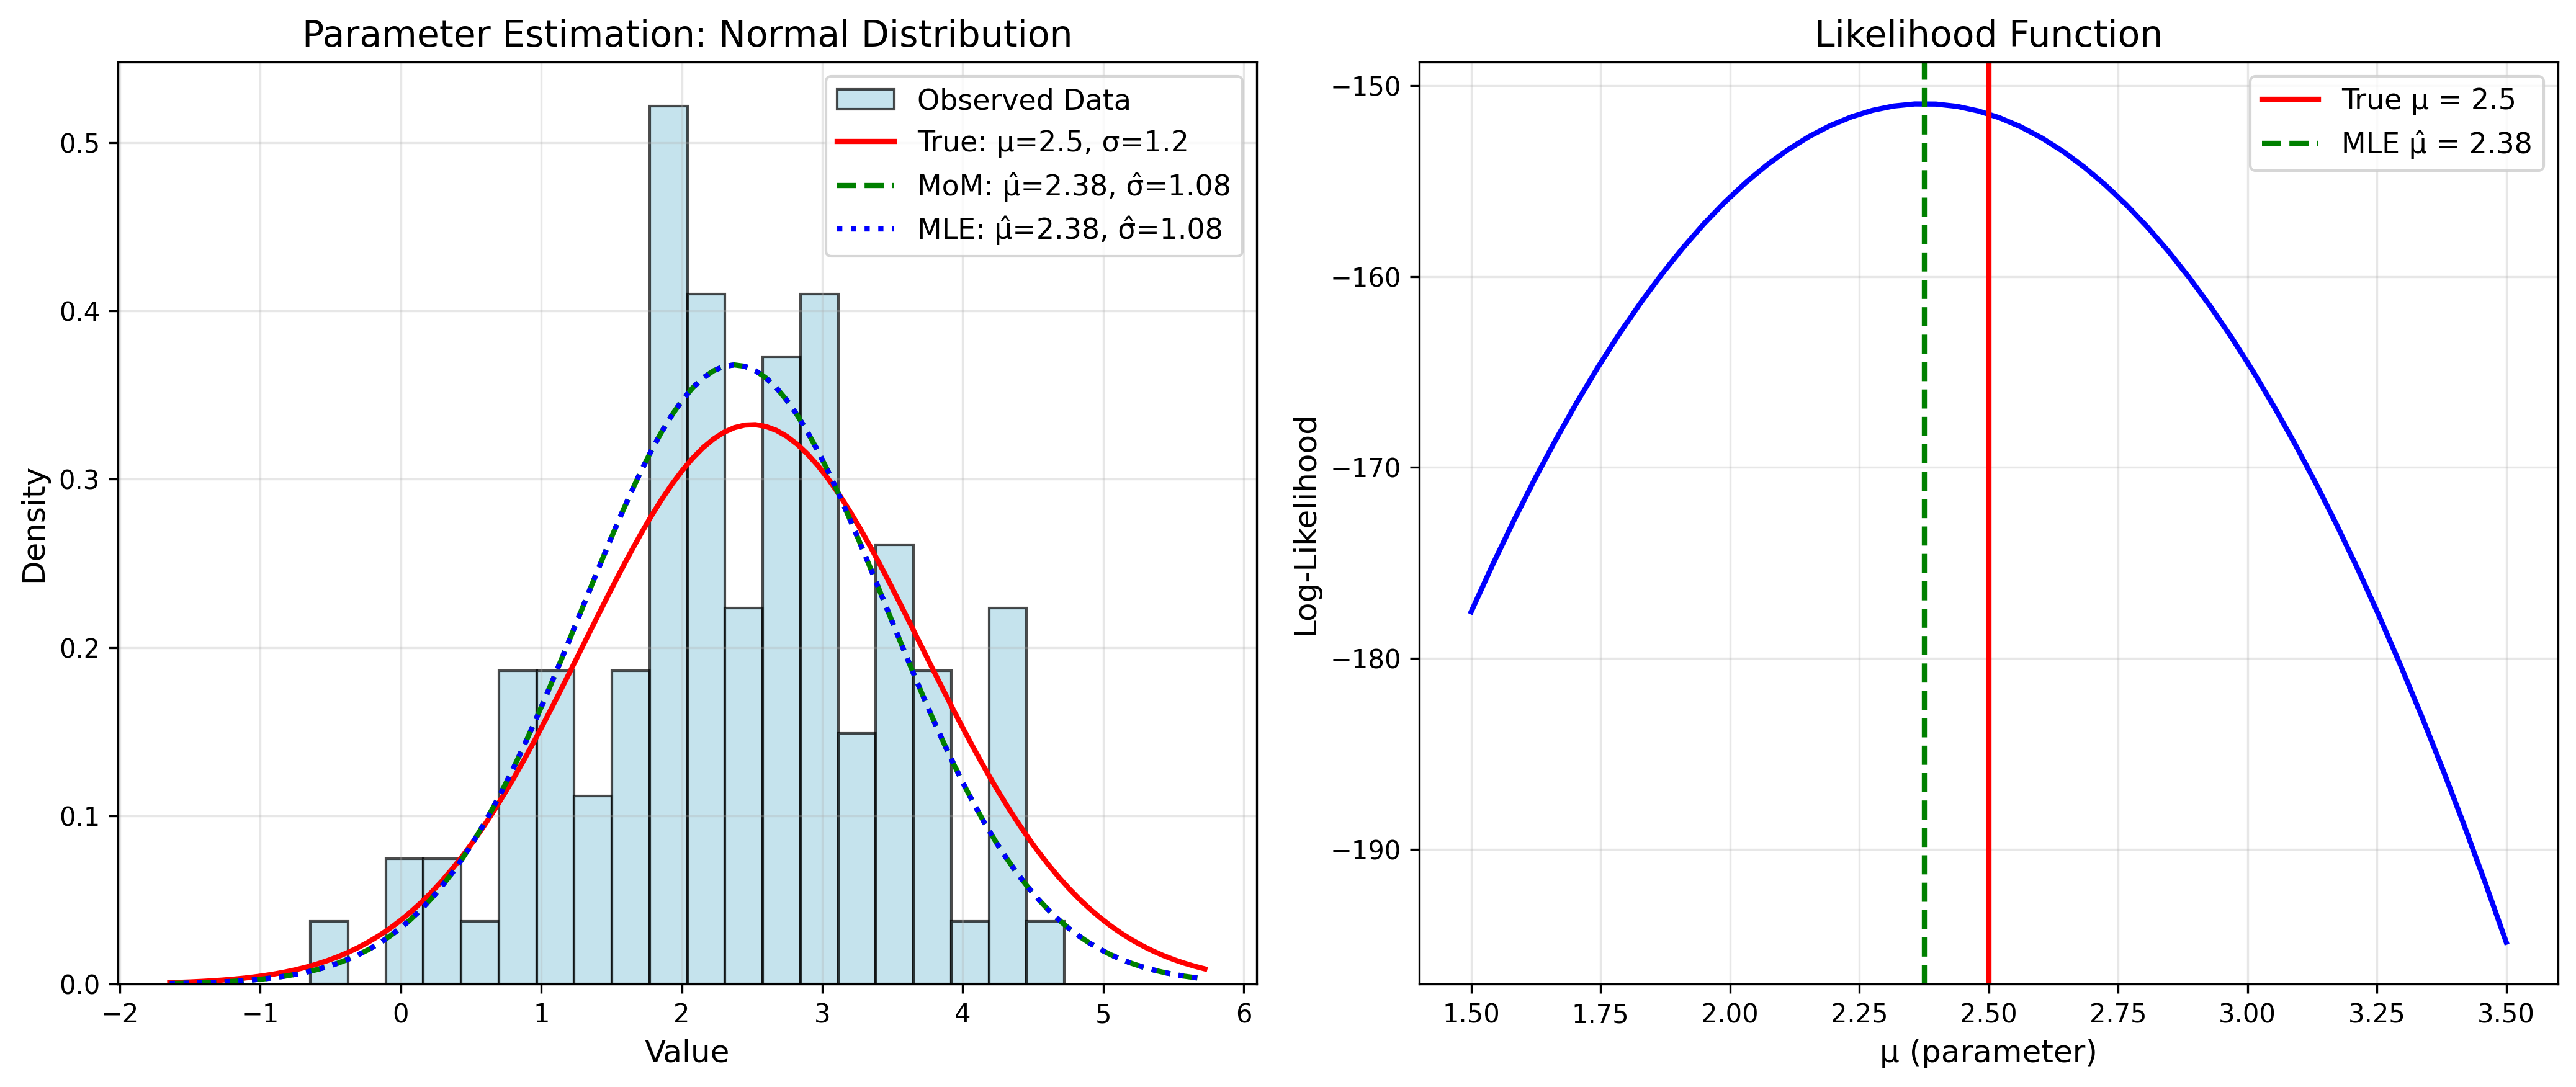
\includegraphics[width=0.6\textwidth]{../figures/parameter_estimation_concept.png}
\end{center}
\end{frame}

\begin{frame}{Why Parameter Estimation Matters}
\begin{columns}[T]
\begin{column}{0.6\textwidth}
\textbf{Machine Learning Applications:}
\begin{itemize}
\setlength{\itemsep}{1pt}
\item \textbf{Supervised Learning:} Estimating model weights
\item \textbf{Unsupervised Learning:} Finding cluster parameters
\item \textbf{Probabilistic Models:} Bayesian inference
\item \textbf{Time Series:} ARIMA parameters
\item \textbf{Deep Learning:} Neural network weights
\end{itemize}
\end{column}
\begin{column}{0.4\textwidth}
\begin{example}
\textbf{Linear Regression:}
Given data $(x_i, y_i)$, estimate:
$$y = \beta_0 + \beta_1 x + \epsilon$$
Find $\hat{\beta}_0, \hat{\beta}_1$ that best fit the data.
\end{example}
\end{column}
\end{columns}


\begin{center}
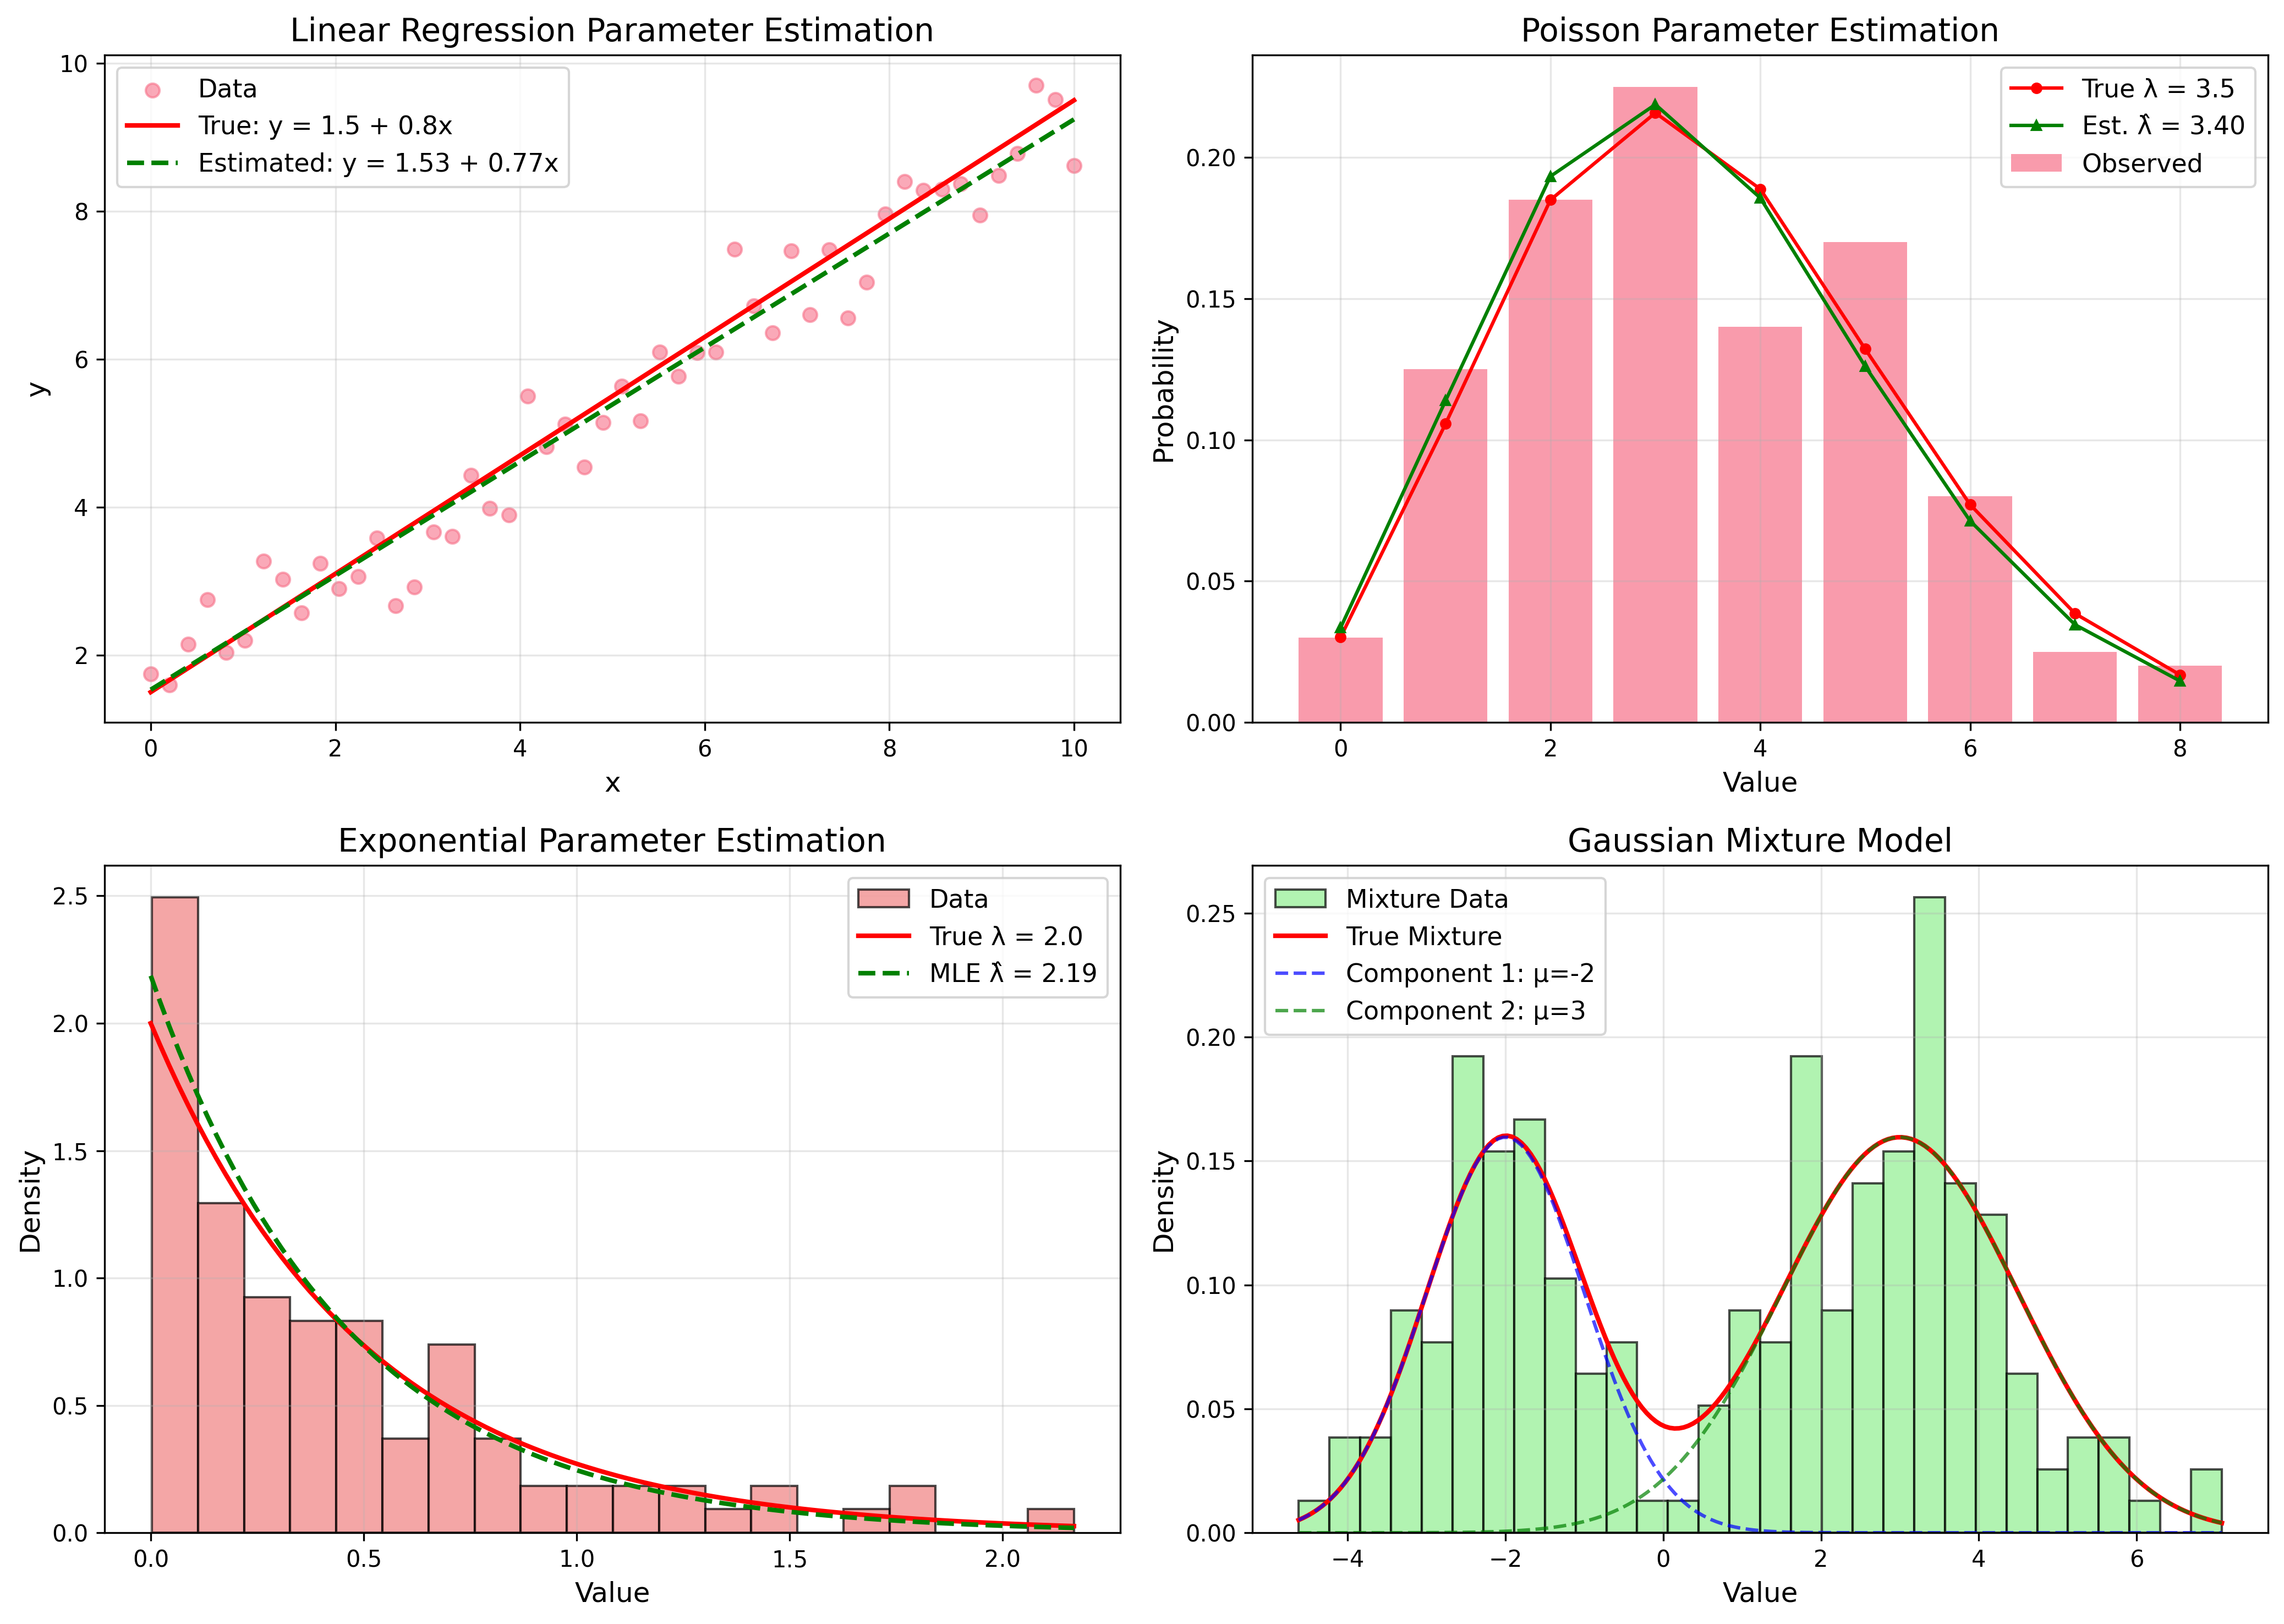
\includegraphics[width=0.6\textwidth]{../figures/ml_applications.png}
\end{center}
\end{frame}

\begin{frame}{Estimation Quality Criteria}
\begin{techblock}{Desirable Properties of Estimators}
\begin{itemize}
\setlength{\itemsep}{2pt}
\item \textbf{Unbiased:} $E[\hat{\theta}] = \theta$
\item \textbf{Consistent:} $\hat{\theta} \xrightarrow{p} \theta$ as $n \to \infty$
\item \textbf{Efficient:} Minimum variance among unbiased estimators
\item \textbf{Sufficient:} Uses all information in the data
\end{itemize}
\end{techblock}


\begin{columns}[T]
\begin{column}{0.5\textwidth}
\textbf{Bias-Variance Tradeoff:}
$$MSE = Bias^2 + Variance + Noise$$
\end{column}
\begin{column}{0.5\textwidth}
\textbf{Cramér-Rao Lower Bound:}
$$Var(\hat{\theta}) \geq \frac{1}{I(\theta)}$$
\end{column}
\end{columns}


\begin{center}
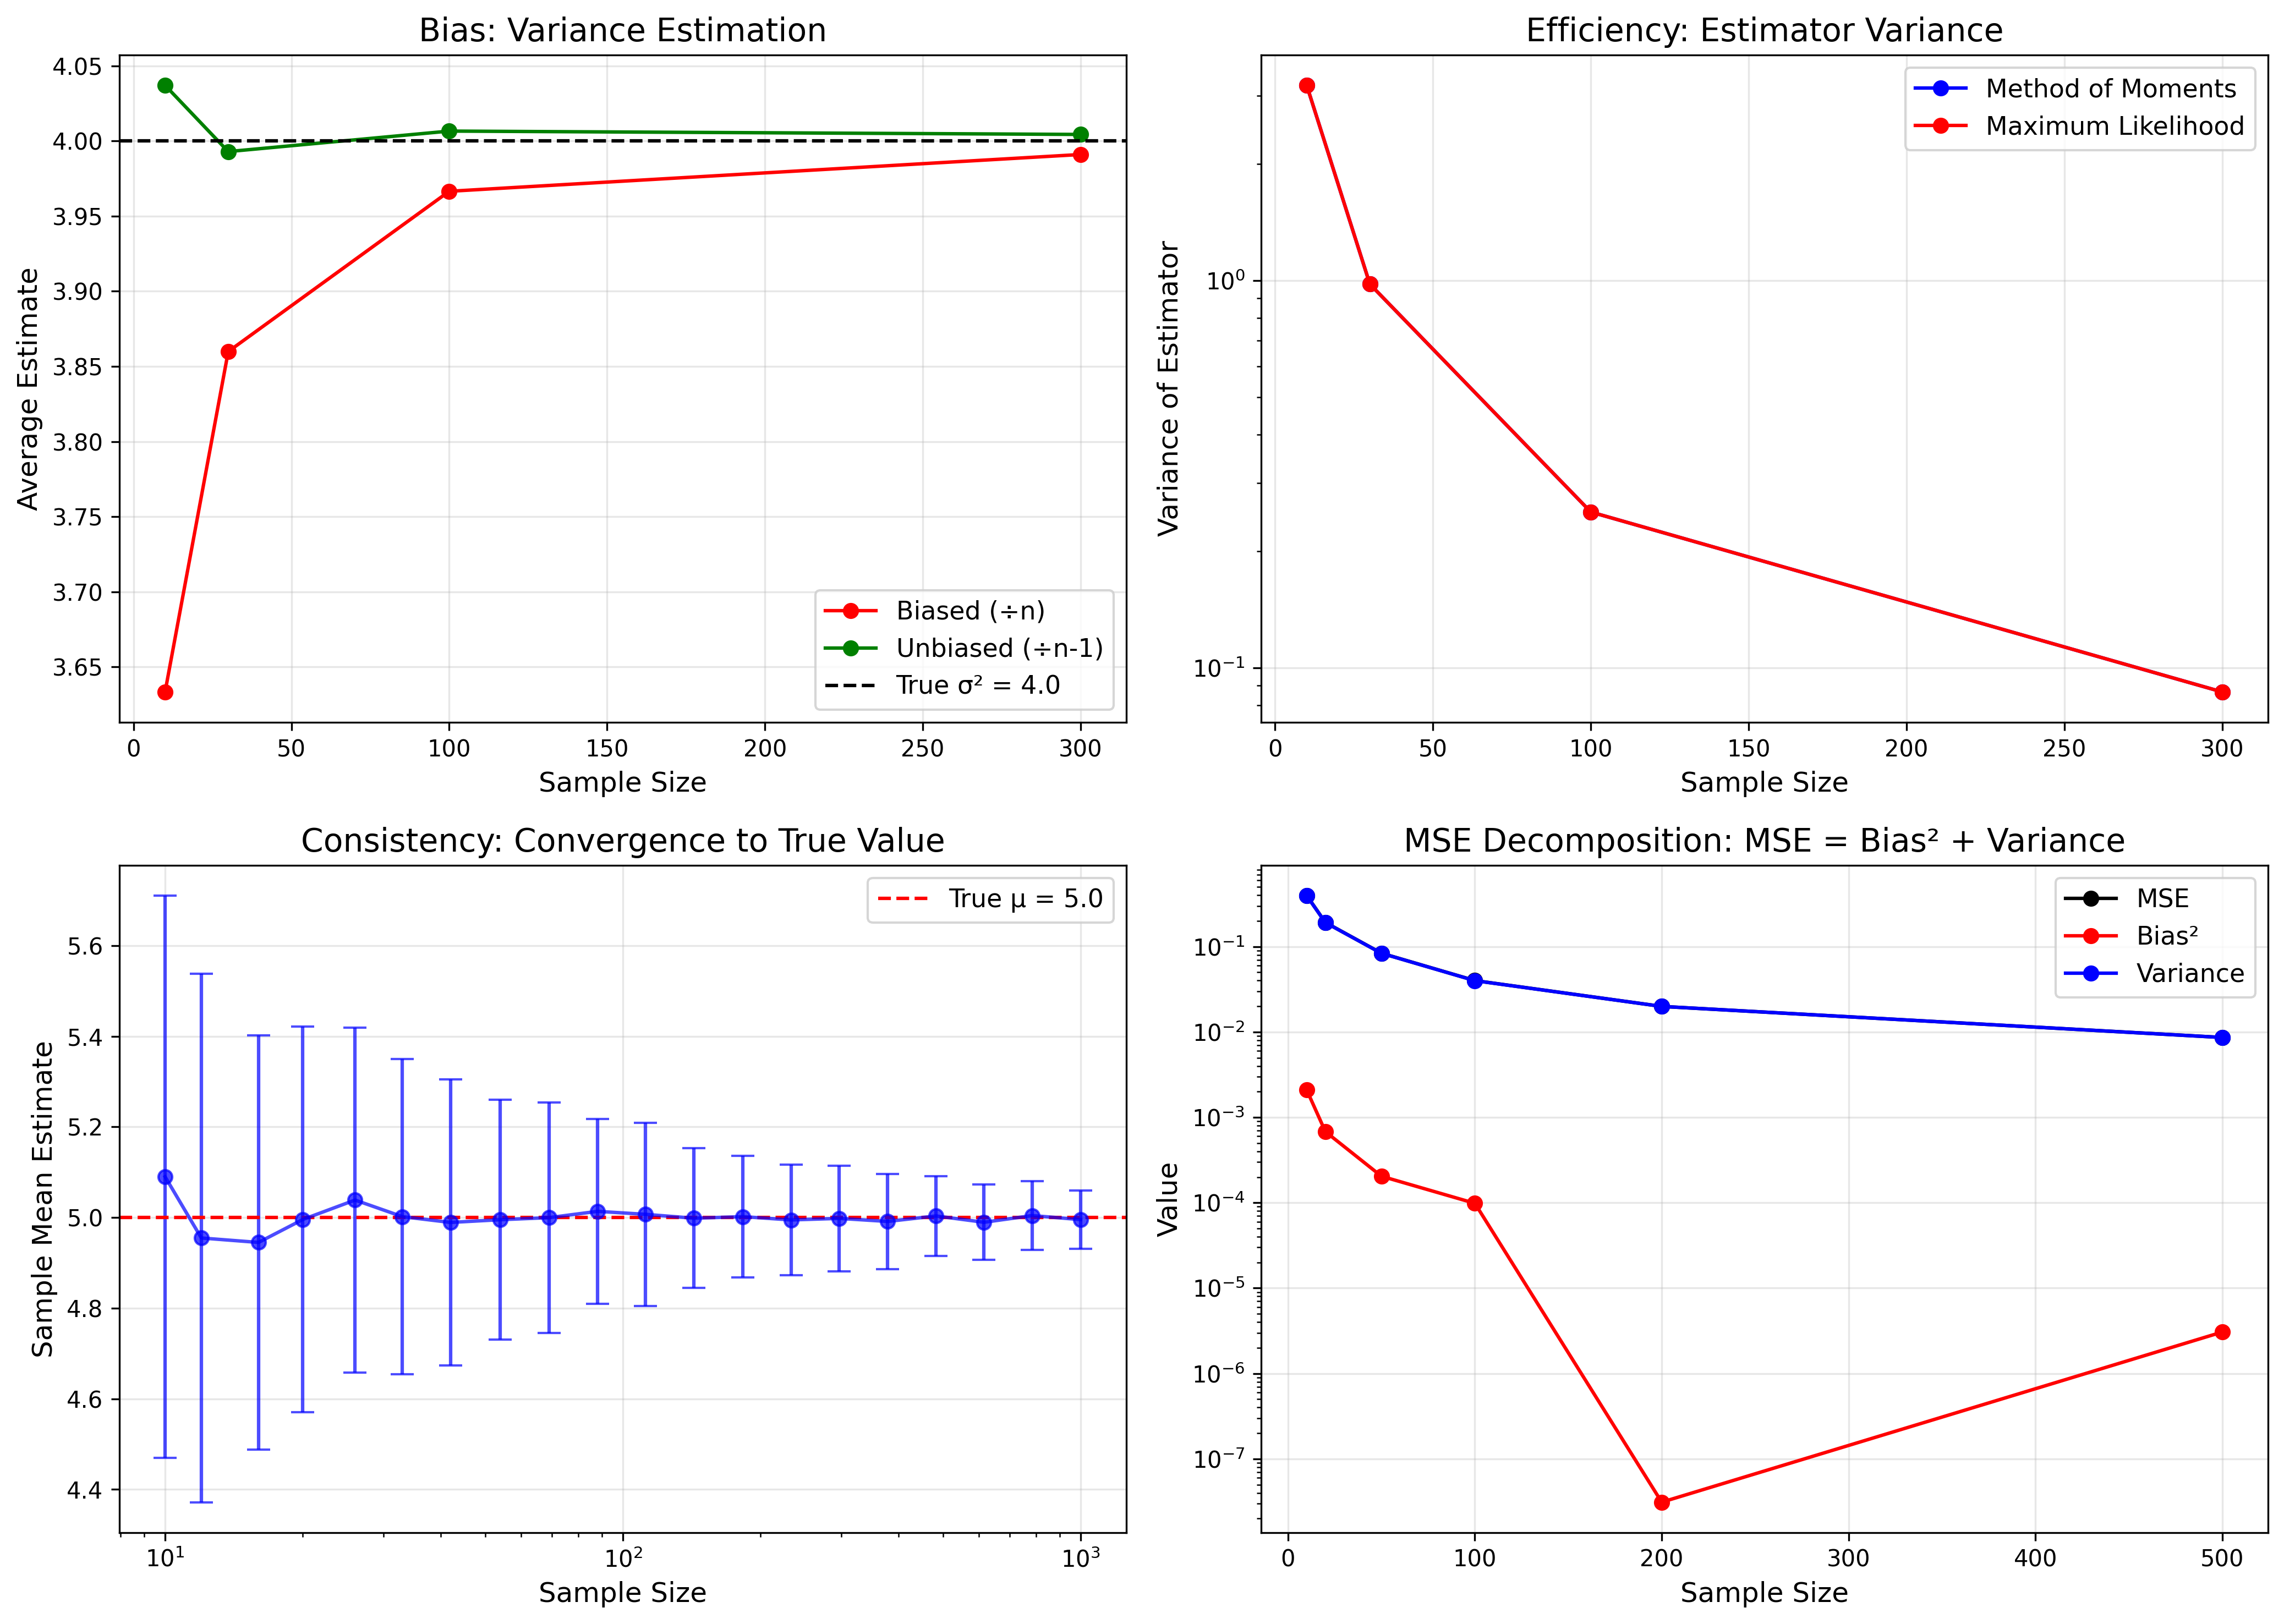
\includegraphics[width=0.6\textwidth]{../figures/estimator_properties.png}
\end{center}
\end{frame}

% SECTION 2: STATISTICAL FOUNDATIONS
\section{Statistical Foundations}

\begin{frame}{Key Concepts and Notation}
\begin{columns}[T]
\begin{column}{0.5\textwidth}
\textbf{Random Variables:}
\begin{itemize}
\setlength{\itemsep}{1pt}
\item $X$: Random variable
\item $x$: Observed value
\item $\theta$: True parameter
\item $\hat{\theta}$: Estimated parameter
\end{itemize}
\end{column}
\begin{column}{0.5\textwidth}
\textbf{Distributions:}
\begin{itemize}
\setlength{\itemsep}{1pt}
\item $f(x|\theta)$: PDF/PMF
\item $F(x|\theta)$: CDF
\item $L(\theta|x)$: Likelihood
\end{itemize}
\end{column}
\end{columns}


\begin{alertblock}{Sample vs Population}
\begin{itemize}
\setlength{\itemsep}{1pt}
\item \textbf{Population:} $\mu = E[X]$, $\sigma^2 = Var(X)$
\item \textbf{Sample:} $\bar{x} = \frac{1}{n}\sum_{i=1}^n x_i$, $s^2 = \frac{1}{n-1}\sum_{i=1}^n (x_i - \bar{x})^2$
\end{itemize}
\end{alertblock}


\begin{example}
For normal distribution $N(\mu, \sigma^2)$:
$$f(x|\mu,\sigma^2) = \frac{1}{\sqrt{2\pi\sigma^2}} \exp\left(-\frac{(x-\mu)^2}{2\sigma^2}\right)$$
\end{example}
\end{frame}

\begin{frame}{Moments and Central Moments}
\begin{techblock}{Definition of Moments}
The $k$-th moment of a random variable $X$:
$$m_k = E[X^k] = \int_{-\infty}^{\infty} x^k f(x) dx$$
\end{techblock}


\begin{columns}[T]
\begin{column}{0.5\textwidth}
\textbf{Raw Moments:}
\begin{itemize}
\setlength{\itemsep}{1pt}
\item $m_1 = E[X] = \mu$ (mean)
\item $m_2 = E[X^2]$
\item $m_3 = E[X^3]$
\item $m_4 = E[X^4]$
\end{itemize}
\end{column}
\begin{column}{0.5\textwidth}
\textbf{Central Moments:}
\begin{itemize}
\setlength{\itemsep}{1pt}
\item $\mu_1 = 0$
\item $\mu_2 = E[(X-\mu)^2] = \sigma^2$ (variance)
\item $\mu_3 = E[(X-\mu)^3]$ (skewness)
\item $\mu_4 = E[(X-\mu)^4]$ (kurtosis)
\end{itemize}
\end{column}
\end{columns}


\begin{example}
For normal distribution $N(\mu, \sigma^2)$:
$m_1 = \mu$, $m_2 = \mu^2 + \sigma^2$, $\mu_2 = \sigma^2$
\end{example}


\begin{center}
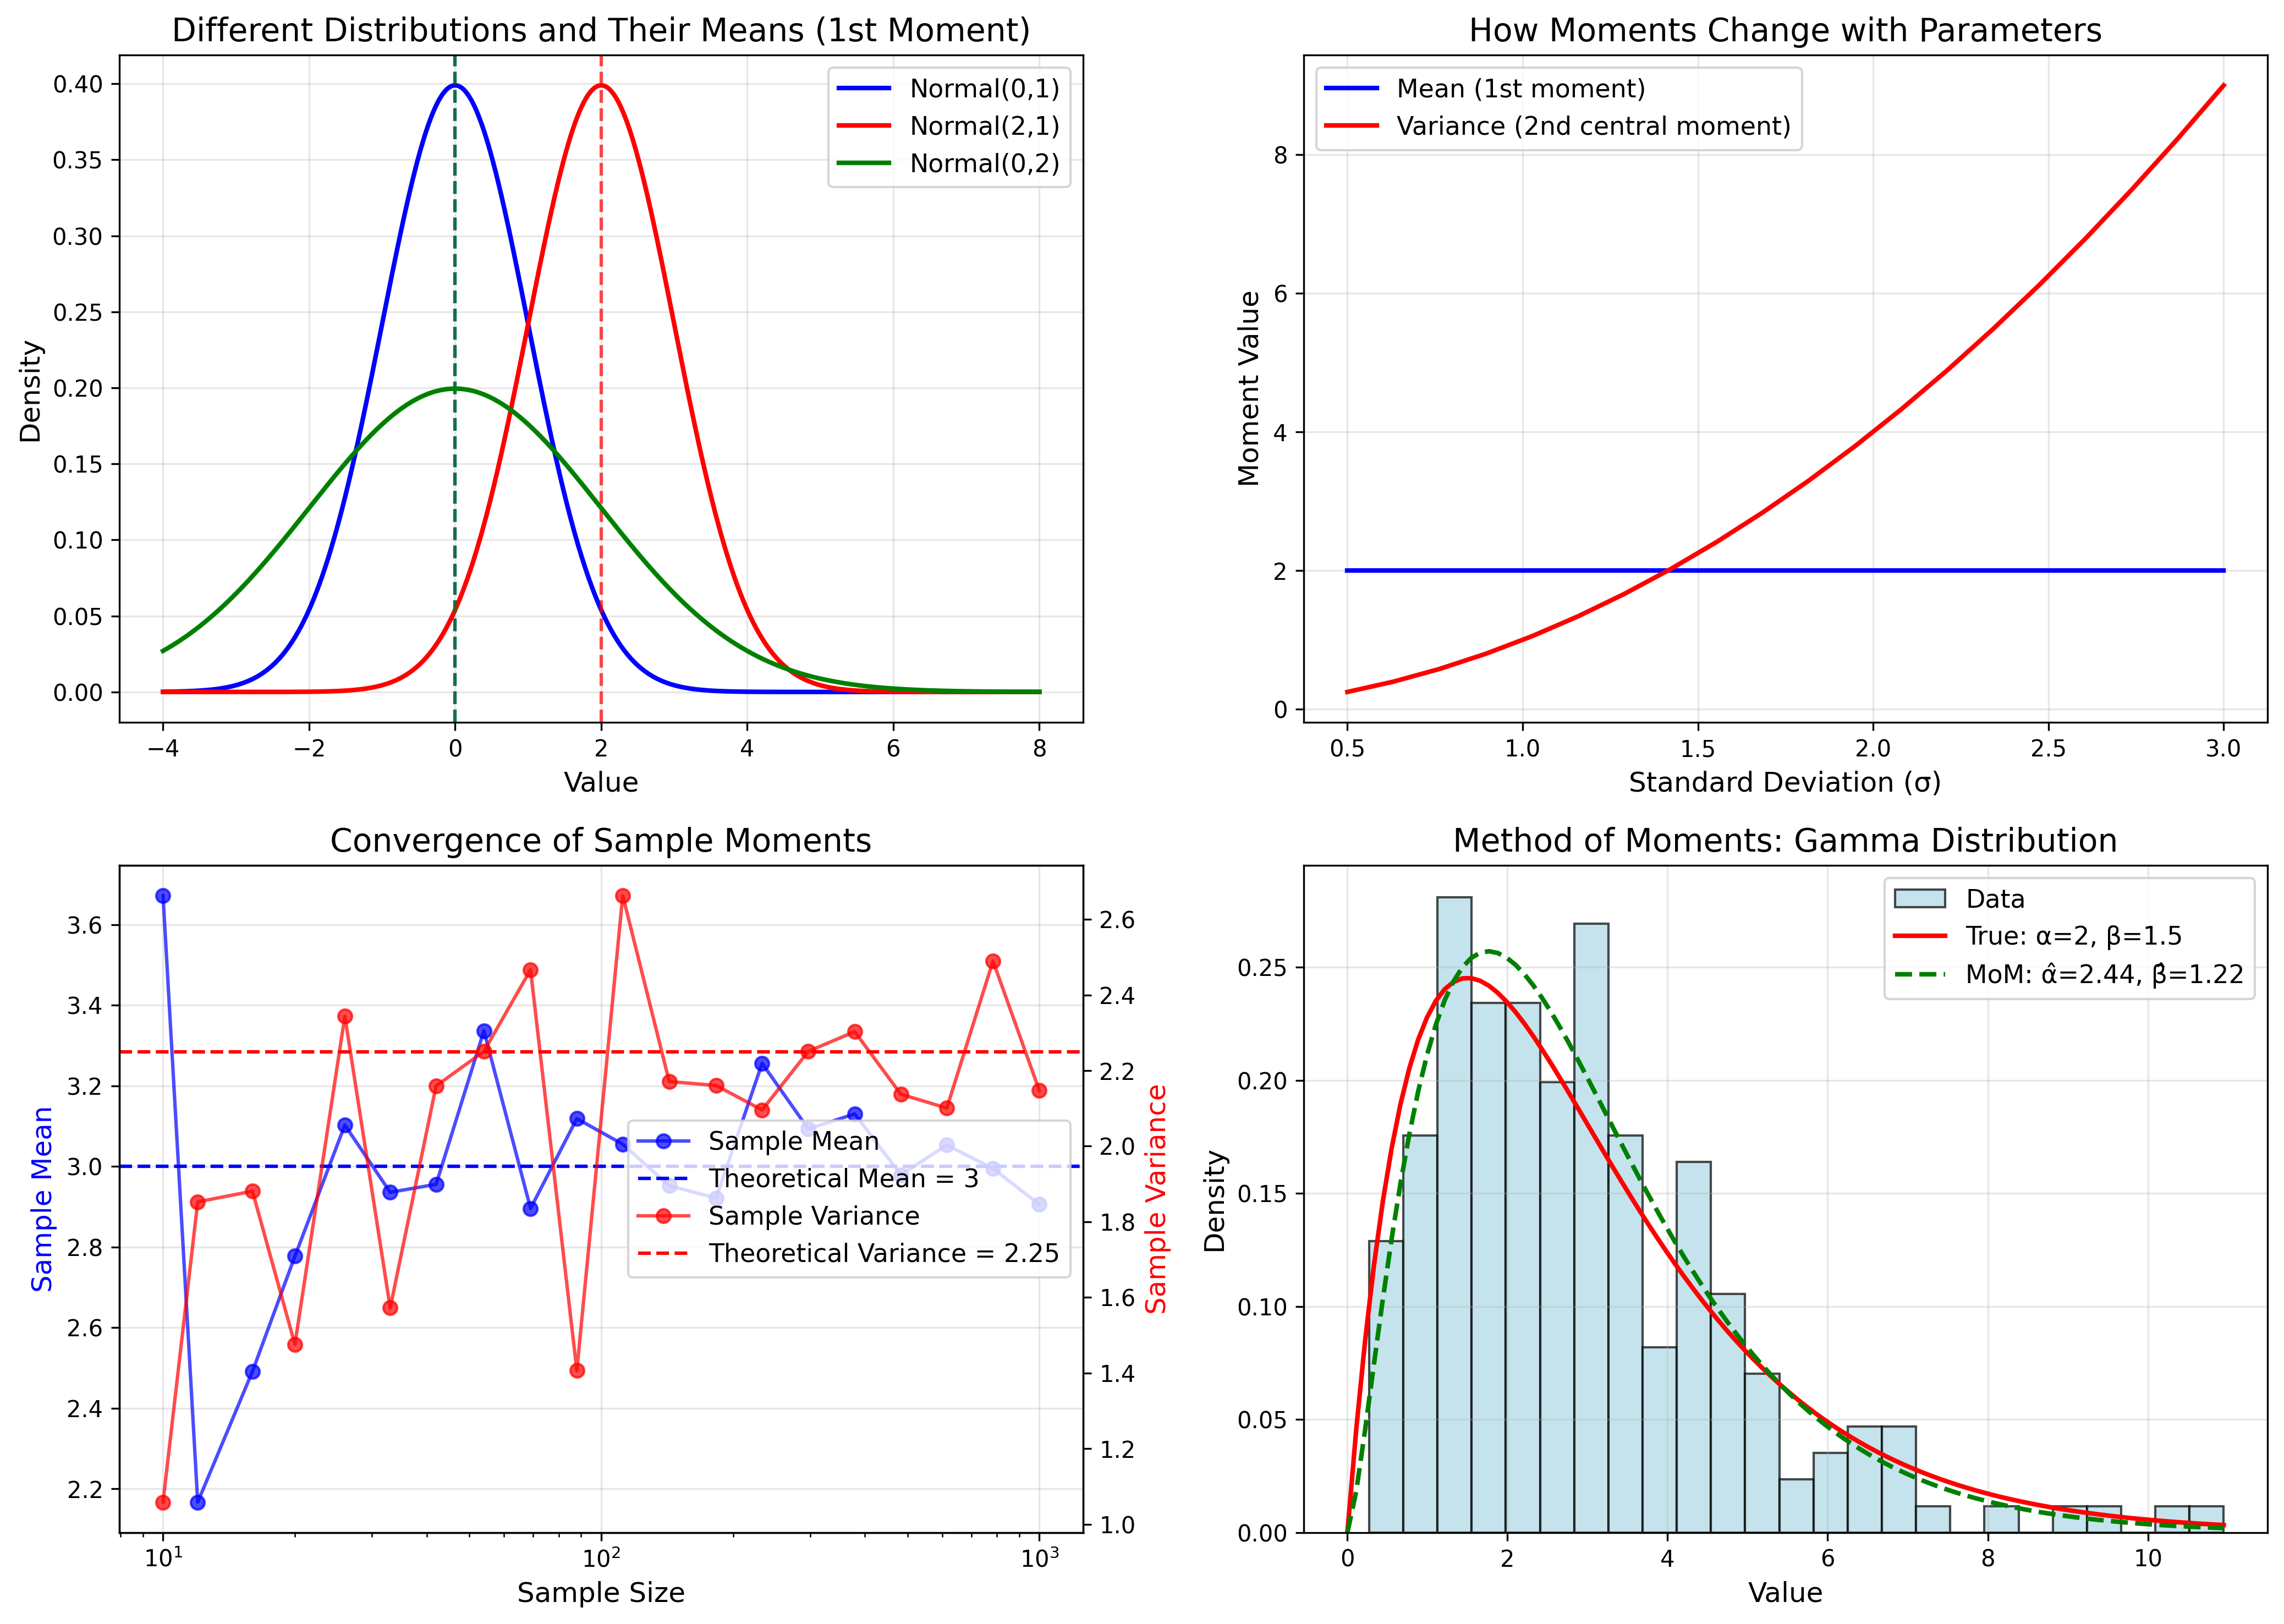
\includegraphics[width=0.6\textwidth]{../figures/moments_illustration.png}
\end{center}
\end{frame}

% SECTION 3: METHOD OF MOMENTS
\section{Method of Moments}

\begin{frame}{Method of Moments: Basic Idea}
\begin{momblock}{Core Principle}
Match sample moments to theoretical moments to estimate parameters.
\end{momblock}


\textbf{Algorithm:}
\begin{enumerate}
\setlength{\itemsep}{1pt}
\item Express theoretical moments in terms of parameters: $m_k(\theta)$
\item Calculate sample moments: $\hat{m}_k = \frac{1}{n}\sum_{i=1}^n x_i^k$
\item Set theoretical = sample: $m_k(\theta) = \hat{m}_k$
\item Solve system of equations for $\hat{\theta}$
\end{enumerate}


\begin{columns}[T]
\begin{column}{0.5\textwidth}
\textbf{For $p$ parameters:}
Use first $p$ moments
$$m_1(\theta) = \hat{m}_1$$
$$m_2(\theta) = \hat{m}_2$$
$$\vdots$$
$$m_p(\theta) = \hat{m}_p$$
\end{column}
\begin{column}{0.5\textwidth}
\begin{alertblock}{Key Insight}
If we can express moments as functions of parameters, we can invert to find parameters from moments.
\end{alertblock}
\end{column}
\end{columns}
\end{frame}

\begin{frame}{MoM Example: Normal Distribution}
\textbf{Problem:} Estimate $\mu$ and $\sigma^2$ for $N(\mu, \sigma^2)$


\begin{columns}[T]
\begin{column}{0.5\textwidth}
\textbf{Step 1: Theoretical moments}
\begin{align}
m_1 &= E[X] = \mu\\
m_2 &= E[X^2] = \mu^2 + \sigma^2
\end{align}
\end{column}
\begin{column}{0.5\textwidth}
\textbf{Step 2: Sample moments}
\begin{align}
\hat{m}_1 &= \frac{1}{n}\sum_{i=1}^n x_i = \bar{x}\\
\hat{m}_2 &= \frac{1}{n}\sum_{i=1}^n x_i^2
\end{align}
\end{column}
\end{columns}


\textbf{Step 3: Set equal and solve}
\begin{align}
\mu &= \bar{x}\\
\mu^2 + \sigma^2 &= \frac{1}{n}\sum_{i=1}^n x_i^2
\end{align}

\textbf{Step 4: Solution}
\begin{align}
\hat{\mu}_{MoM} &= \bar{x}\\
\hat{\sigma}^2_{MoM} &= \frac{1}{n}\sum_{i=1}^n x_i^2 - \bar{x}^2 = \frac{1}{n}\sum_{i=1}^n (x_i - \bar{x})^2
\end{align}
\end{frame}

\begin{frame}{MoM Example: Poisson Distribution}
\textbf{Problem:} Estimate $\lambda$ for Poisson($\lambda$)


\begin{columns}[T]
\begin{column}{0.6\textwidth}
\textbf{Theoretical moment:}
For Poisson distribution:
$$E[X] = \lambda$$

\textbf{Sample moment:}
$$\hat{m}_1 = \bar{x} = \frac{1}{n}\sum_{i=1}^n x_i$$

\textbf{MoM Estimate:}
$$\hat{\lambda}_{MoM} = \bar{x}$$
\end{column}
\begin{column}{0.4\textwidth}
\begin{example}
Data: [2, 1, 3, 0, 2, 1, 4, 1]

Sample mean:
$$\bar{x} = \frac{14}{8} = 1.75$$

MoM estimate:
$$\hat{\lambda} = 1.75$$
\end{example}
\end{column}
\end{columns}


\begin{center}
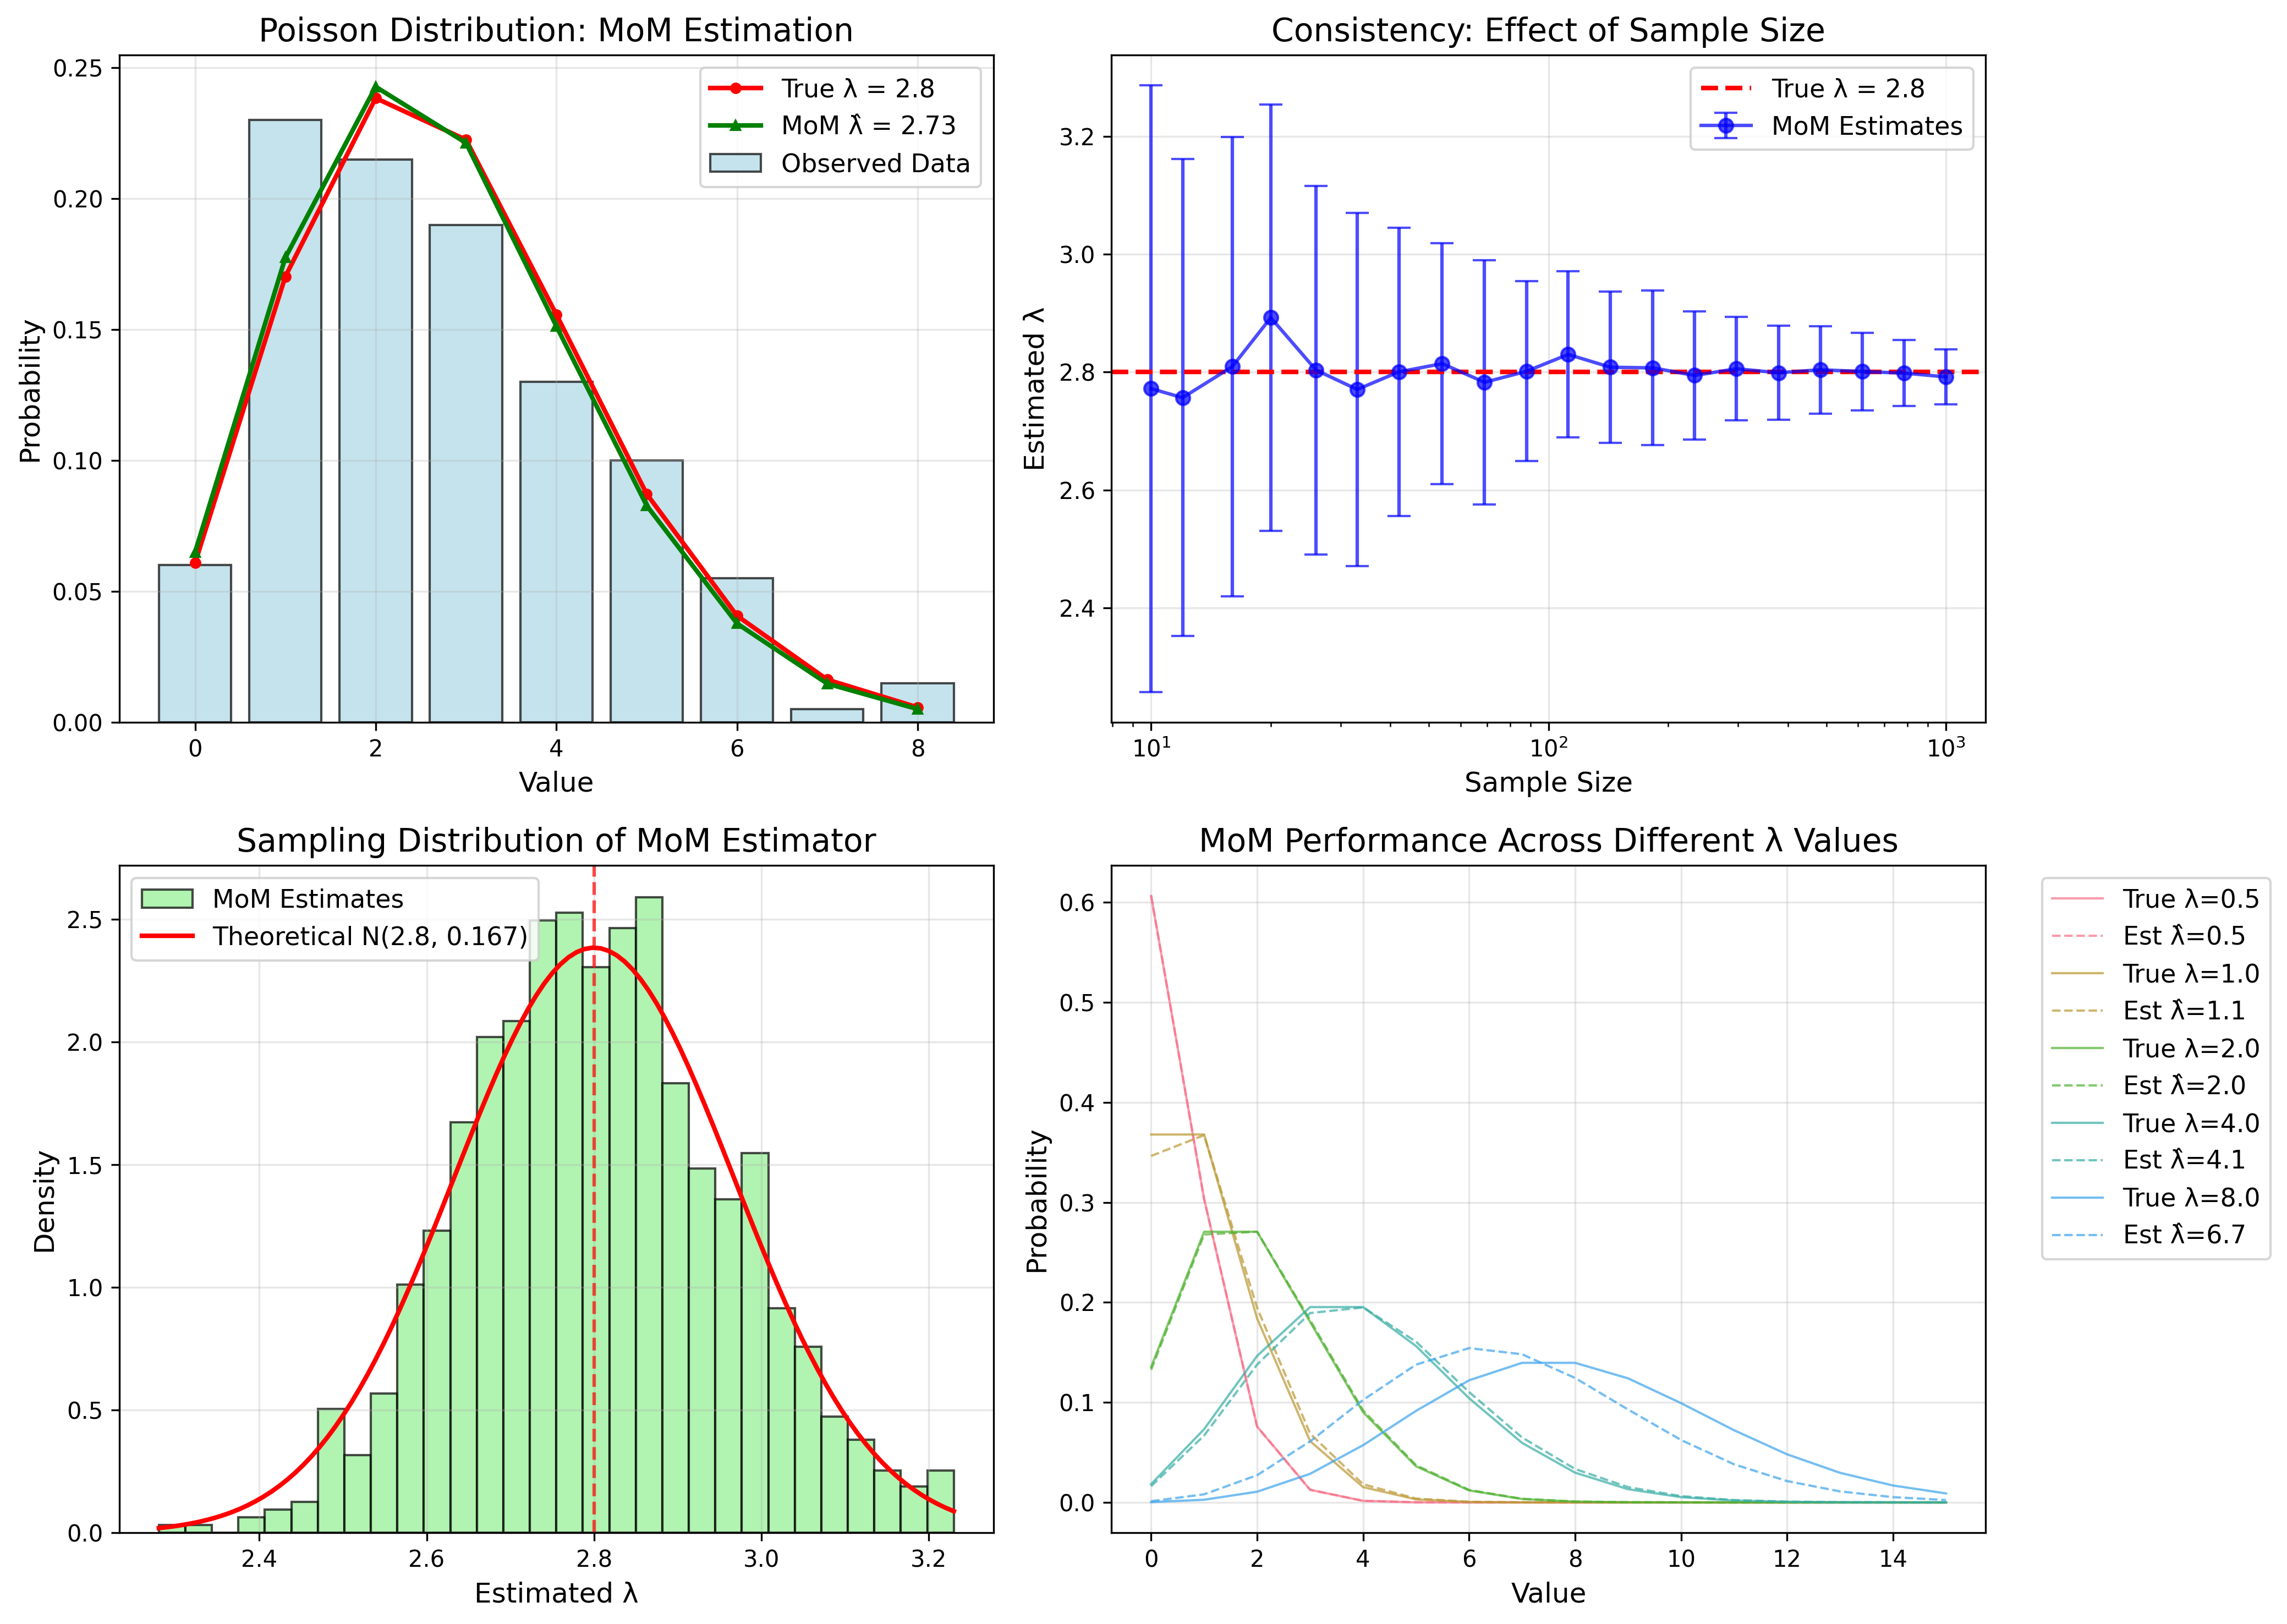
\includegraphics[width=0.6\textwidth]{../figures/mom_poisson_example.png}
\end{center}
\end{frame}

\begin{frame}{MoM Example: Gamma Distribution}
\textbf{Problem:} Estimate $\alpha$ and $\beta$ for Gamma($\alpha, \beta$)


\begin{columns}[T]
\begin{column}{0.5\textwidth}
\textbf{Theoretical moments:}
\begin{align}
E[X] &= \alpha\beta\\
Var(X) &= \alpha\beta^2
\end{align}

Also: $E[X^2] = Var(X) + (E[X])^2 = \alpha\beta^2 + \alpha^2\beta^2$
\end{column}
\begin{column}{0.5\textwidth}
\textbf{Sample moments:}
\begin{align}
\hat{m}_1 &= \bar{x}\\
\hat{m}_2 &= \frac{1}{n}\sum_{i=1}^n x_i^2
\end{align}

Sample variance:
$$\hat{\sigma}^2 = \hat{m}_2 - \hat{m}_1^2$$
\end{column}
\end{columns}


\textbf{Setting moments equal:}
\begin{align}
\alpha\beta &= \bar{x}\\
\alpha\beta^2 &= \hat{\sigma}^2
\end{align}

\textbf{MoM Estimates:}
$$\hat{\beta}_{MoM} = \frac{\hat{\sigma}^2}{\bar{x}}, \quad \hat{\alpha}_{MoM} = \frac{\bar{x}^2}{\hat{\sigma}^2}$$
\end{frame}

\begin{frame}{Properties of Method of Moments}
\begin{columns}[T]
\begin{column}{0.5\textwidth}
\begin{block}{Advantages}
\begin{itemize}
\setlength{\itemsep}{1pt}
\item \textbf{Simple:} Easy to compute
\item \textbf{Consistent:} $\hat{\theta} \to \theta$ as $n \to \infty$
\item \textbf{General:} Works for any distribution
\item \textbf{Intuitive:} Matches sample to theory
\end{itemize}
\end{block}
\end{column}
\begin{column}{0.5\textwidth}
\begin{alertblock}{Disadvantages}
\begin{itemize}
\setlength{\itemsep}{1pt}
\item \textbf{Not optimal:} Higher variance than MLE
\item \textbf{Existence:} Solutions may not exist
\item \textbf{Uniqueness:} Multiple solutions possible
\item \textbf{Boundary:} May give invalid estimates
\end{itemize}
\end{alertblock}
\end{column}
\end{columns}


\begin{techblock}{Asymptotic Distribution}
Under regularity conditions:
$$\sqrt{n}(\hat{\theta}_{MoM} - \theta) \xrightarrow{d} N(0, \Sigma)$$
where $\Sigma$ depends on the moments and their derivatives.
\end{techblock}


\begin{center}

\includegraphics[width=0.6\textwidth]{../figures/mom_properties.png}
\end{center}
\end{frame}

% SECTION 4: MAXIMUM LIKELIHOOD ESTIMATION
\section{Maximum Likelihood Estimation}

\begin{frame}{Maximum Likelihood: Basic Idea}
\begin{mleblock}{Core Principle}
Find parameter values that make the observed data most likely.
\end{mleblock}


\textbf{Likelihood Function:}
For independent observations $x_1, x_2, \ldots, x_n$:
$$L(\theta) = L(\theta | x_1, \ldots, x_n) = \prod_{i=1}^n f(x_i | \theta)$$

\textbf{Log-Likelihood:}
$$\ell(\theta) = \log L(\theta) = \sum_{i=1}^n \log f(x_i | \theta)$$


\begin{alertblock}{Maximum Likelihood Estimator (MLE)}
$$\hat{\theta}_{MLE} = \arg\max_\theta L(\theta) = \arg\max_\theta \ell(\theta)$$
\end{alertblock}


\begin{center}
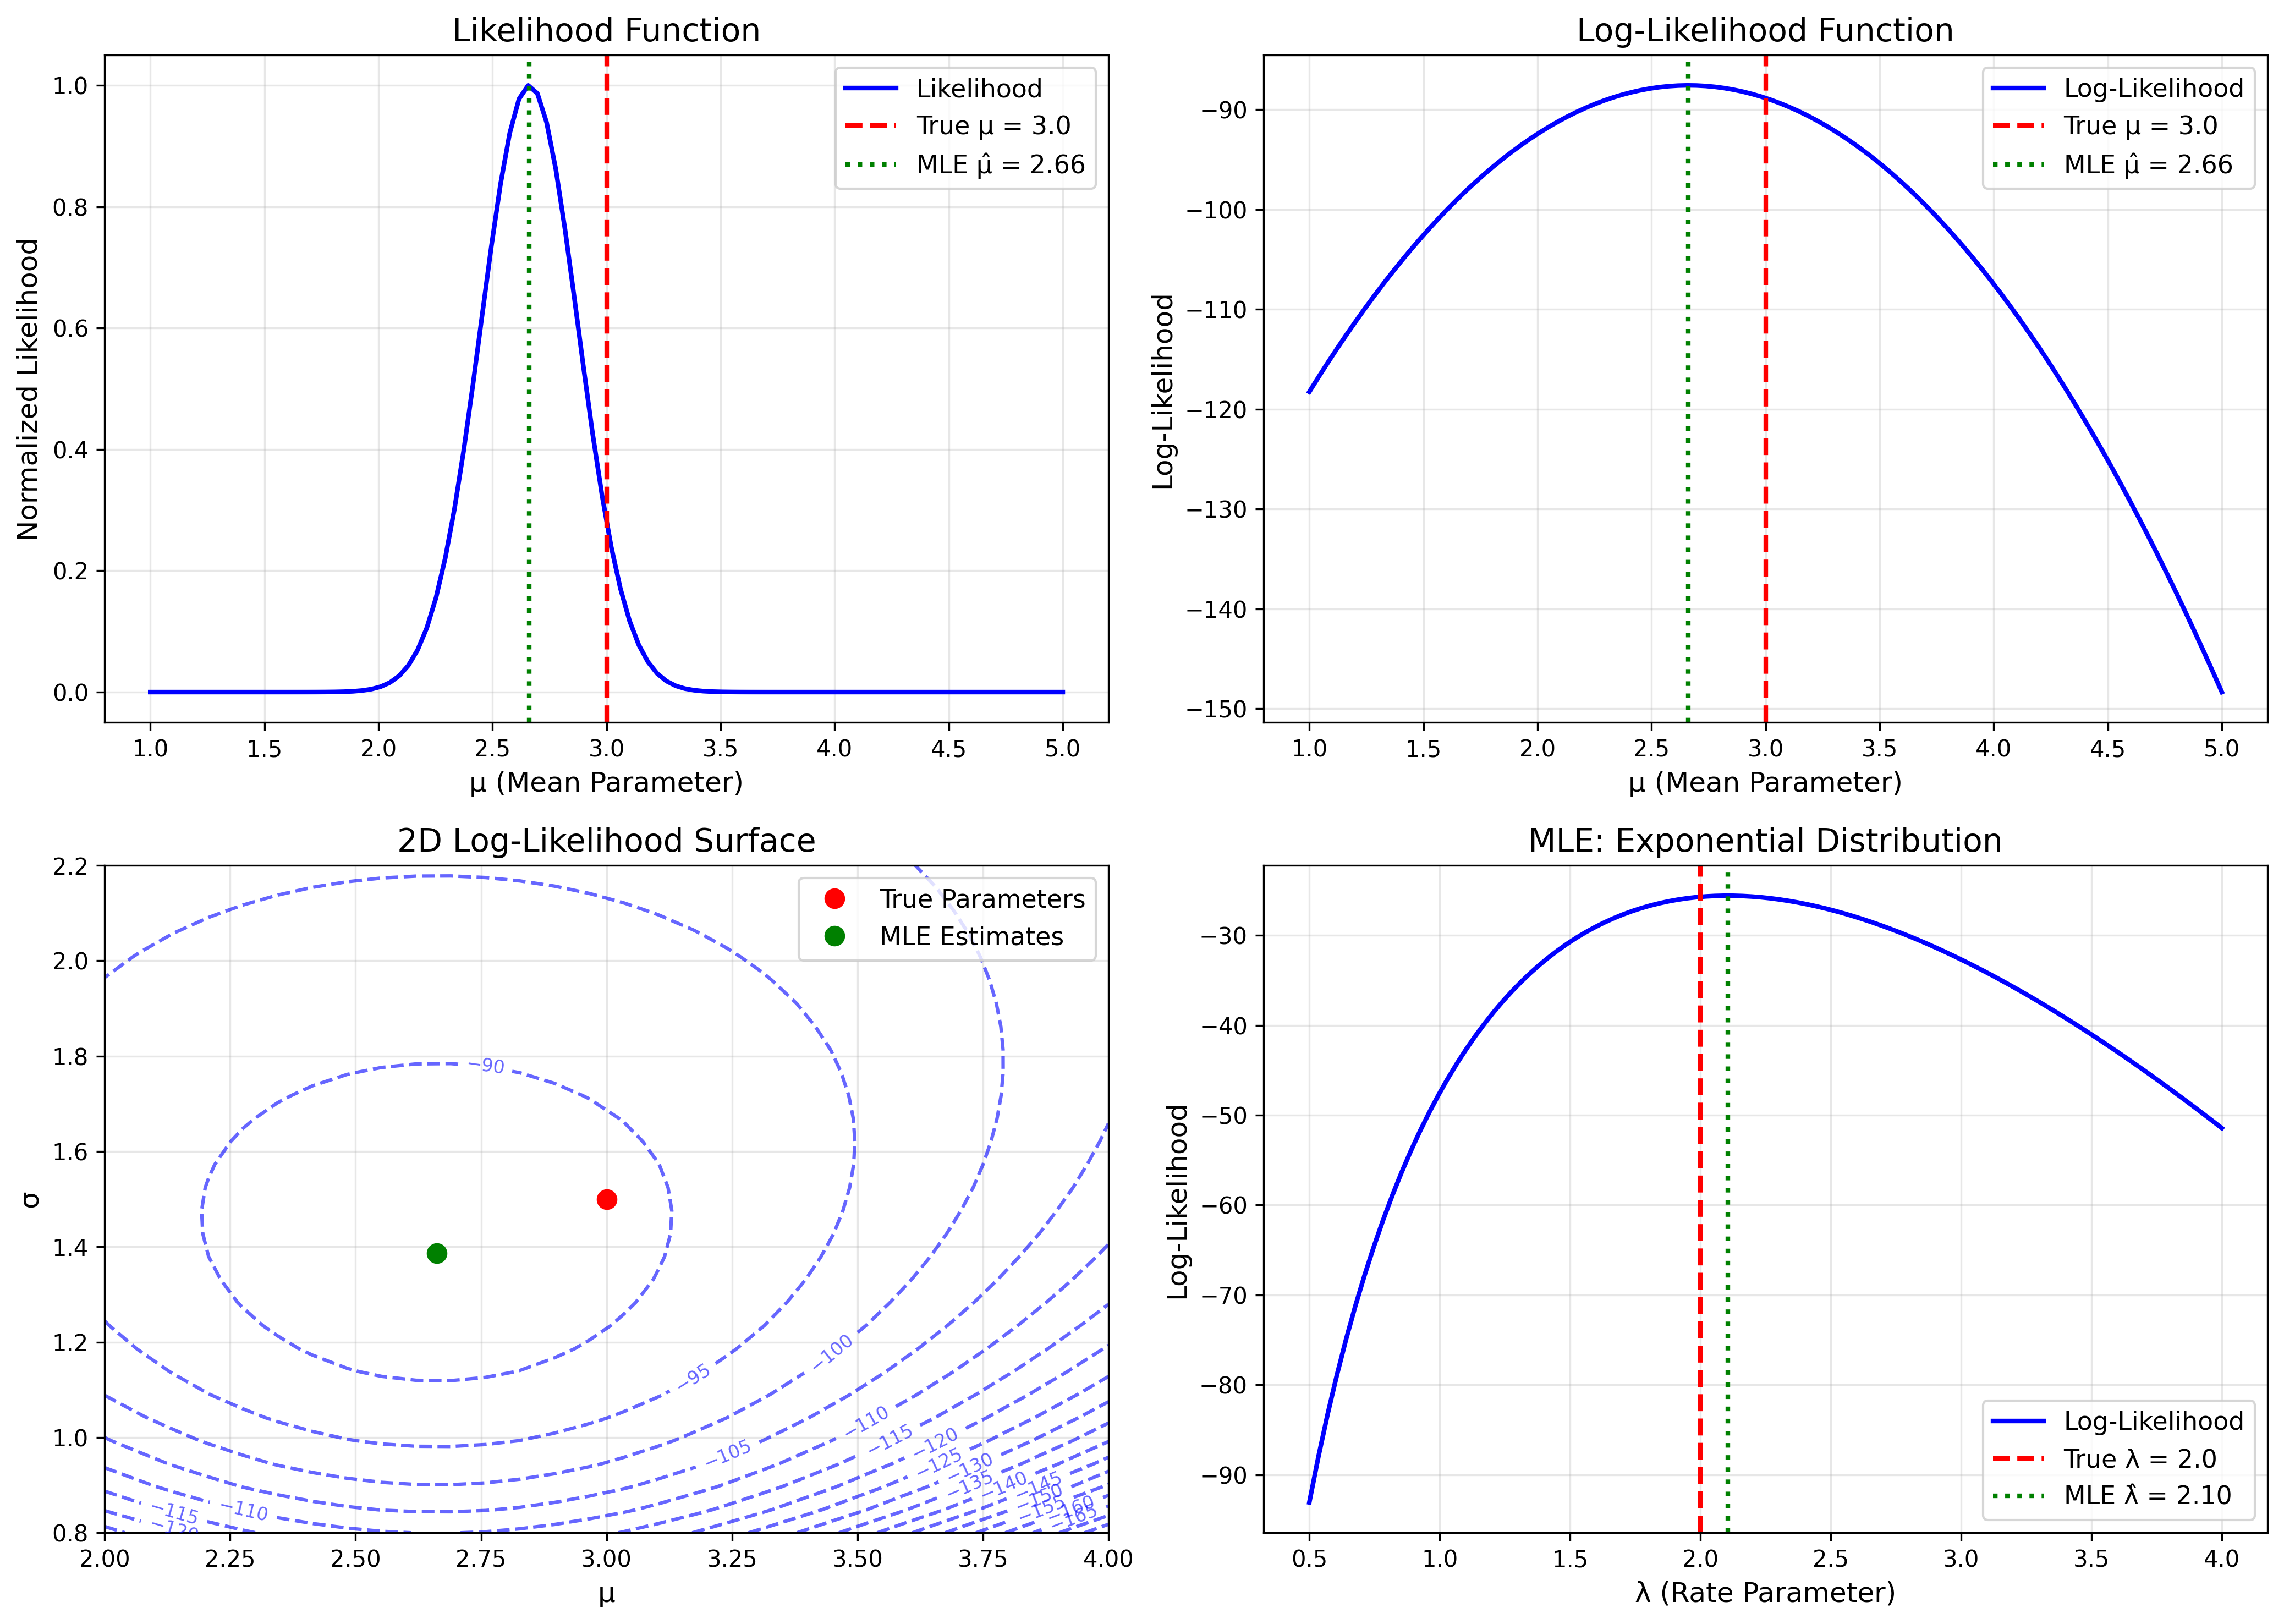
\includegraphics[width=0.6\textwidth]{../figures/likelihood_concept.png}
\end{center}
\end{frame}

\begin{frame}{Finding the MLE: Calculus Approach}
\textbf{Method 1: Differentiation}

For continuous parameter space, solve:
$$\frac{d\ell(\theta)}{d\theta} = 0$$

\textbf{Score Function:}
$$S(\theta) = \frac{d\ell(\theta)}{d\theta} = \sum_{i=1}^n \frac{d\log f(x_i|\theta)}{d\theta}$$


\begin{columns}[T]
\begin{column}{0.5\textwidth}
\textbf{For vector parameters $\boldsymbol{\theta}$:}
$$\nabla_{\boldsymbol{\theta}} \ell(\boldsymbol{\theta}) = \mathbf{0}$$

This gives a system of equations to solve.
\end{column}
\begin{column}{0.5\textwidth}
\textbf{Second-order condition:}
$$\frac{d^2\ell(\theta)}{d\theta^2} < 0$$

Ensures we have a maximum, not minimum.
\end{column}
\end{columns}


\begin{example}
For normal distribution with known $\sigma^2$:
$$\frac{d\ell(\mu)}{d\mu} = \frac{1}{\sigma^2}\sum_{i=1}^n (x_i - \mu) = 0$$
$$\Rightarrow \hat{\mu}_{MLE} = \bar{x}$$
\end{example}
\end{frame}

\begin{frame}{MLE Example: Normal Distribution}
\textbf{Problem:} Estimate $\mu$ and $\sigma^2$ for $N(\mu, \sigma^2)$


\textbf{Log-likelihood:}
\begin{align}
\ell(\mu, \sigma^2) &= \sum_{i=1}^n \log f(x_i | \mu, \sigma^2)\\
&= \sum_{i=1}^n \left[-\frac{1}{2}\log(2\pi) - \frac{1}{2}\log(\sigma^2) - \frac{(x_i-\mu)^2}{2\sigma^2}\right]\\
&= -\frac{n}{2}\log(2\pi) - \frac{n}{2}\log(\sigma^2) - \frac{1}{2\sigma^2}\sum_{i=1}^n(x_i-\mu)^2
\end{align}

\textbf{Taking derivatives:}
\begin{align}
\frac{\partial \ell}{\partial \mu} &= \frac{1}{\sigma^2}\sum_{i=1}^n(x_i - \mu) = 0\\
\frac{\partial \ell}{\partial \sigma^2} &= -\frac{n}{2\sigma^2} + \frac{1}{2(\sigma^2)^2}\sum_{i=1}^n(x_i-\mu)^2 = 0
\end{align}

\textbf{MLE Solutions:}
$$\hat{\mu}_{MLE} = \bar{x}, \quad \hat{\sigma}^2_{MLE} = \frac{1}{n}\sum_{i=1}^n(x_i - \bar{x})^2$$
\end{frame}

\begin{frame}{MLE Example: Poisson Distribution}
\textbf{Problem:} Estimate $\lambda$ for Poisson($\lambda$)


\textbf{PMF:} $P(X = k) = \frac{\lambda^k e^{-\lambda}}{k!}$

\textbf{Log-likelihood:}
\begin{align}
\ell(\lambda) &= \sum_{i=1}^n \log P(X_i = x_i | \lambda)\\
&= \sum_{i=1}^n \left[x_i \log \lambda - \lambda - \log(x_i!)\right]\\
&= \log \lambda \sum_{i=1}^n x_i - n\lambda - \sum_{i=1}^n \log(x_i!)
\end{align}

\textbf{Score function:}
$$\frac{d\ell(\lambda)}{d\lambda} = \frac{1}{\lambda}\sum_{i=1}^n x_i - n = 0$$

\textbf{MLE Solution:}
$$\hat{\lambda}_{MLE} = \frac{1}{n}\sum_{i=1}^n x_i = \bar{x}$$

\begin{alertblock}{Note}
For Poisson distribution, MLE and MoM give the same result!
\end{alertblock}
\end{frame}

\begin{frame}{MLE Example: Exponential Distribution}
\textbf{Problem:} Estimate $\lambda$ for Exponential($\lambda$)


\textbf{PDF:} $f(x|\lambda) = \lambda e^{-\lambda x}$ for $x \geq 0$

\textbf{Log-likelihood:}
\begin{align}
\ell(\lambda) &= \sum_{i=1}^n \log(\lambda e^{-\lambda x_i})\\
&= \sum_{i=1}^n [\log \lambda - \lambda x_i]\\
&= n \log \lambda - \lambda \sum_{i=1}^n x_i
\end{align}

\textbf{Score function:}
$$\frac{d\ell(\lambda)}{d\lambda} = \frac{n}{\lambda} - \sum_{i=1}^n x_i = 0$$

\textbf{MLE Solution:}
$$\hat{\lambda}_{MLE} = \frac{n}{\sum_{i=1}^n x_i} = \frac{1}{\bar{x}}$$


\begin{center}
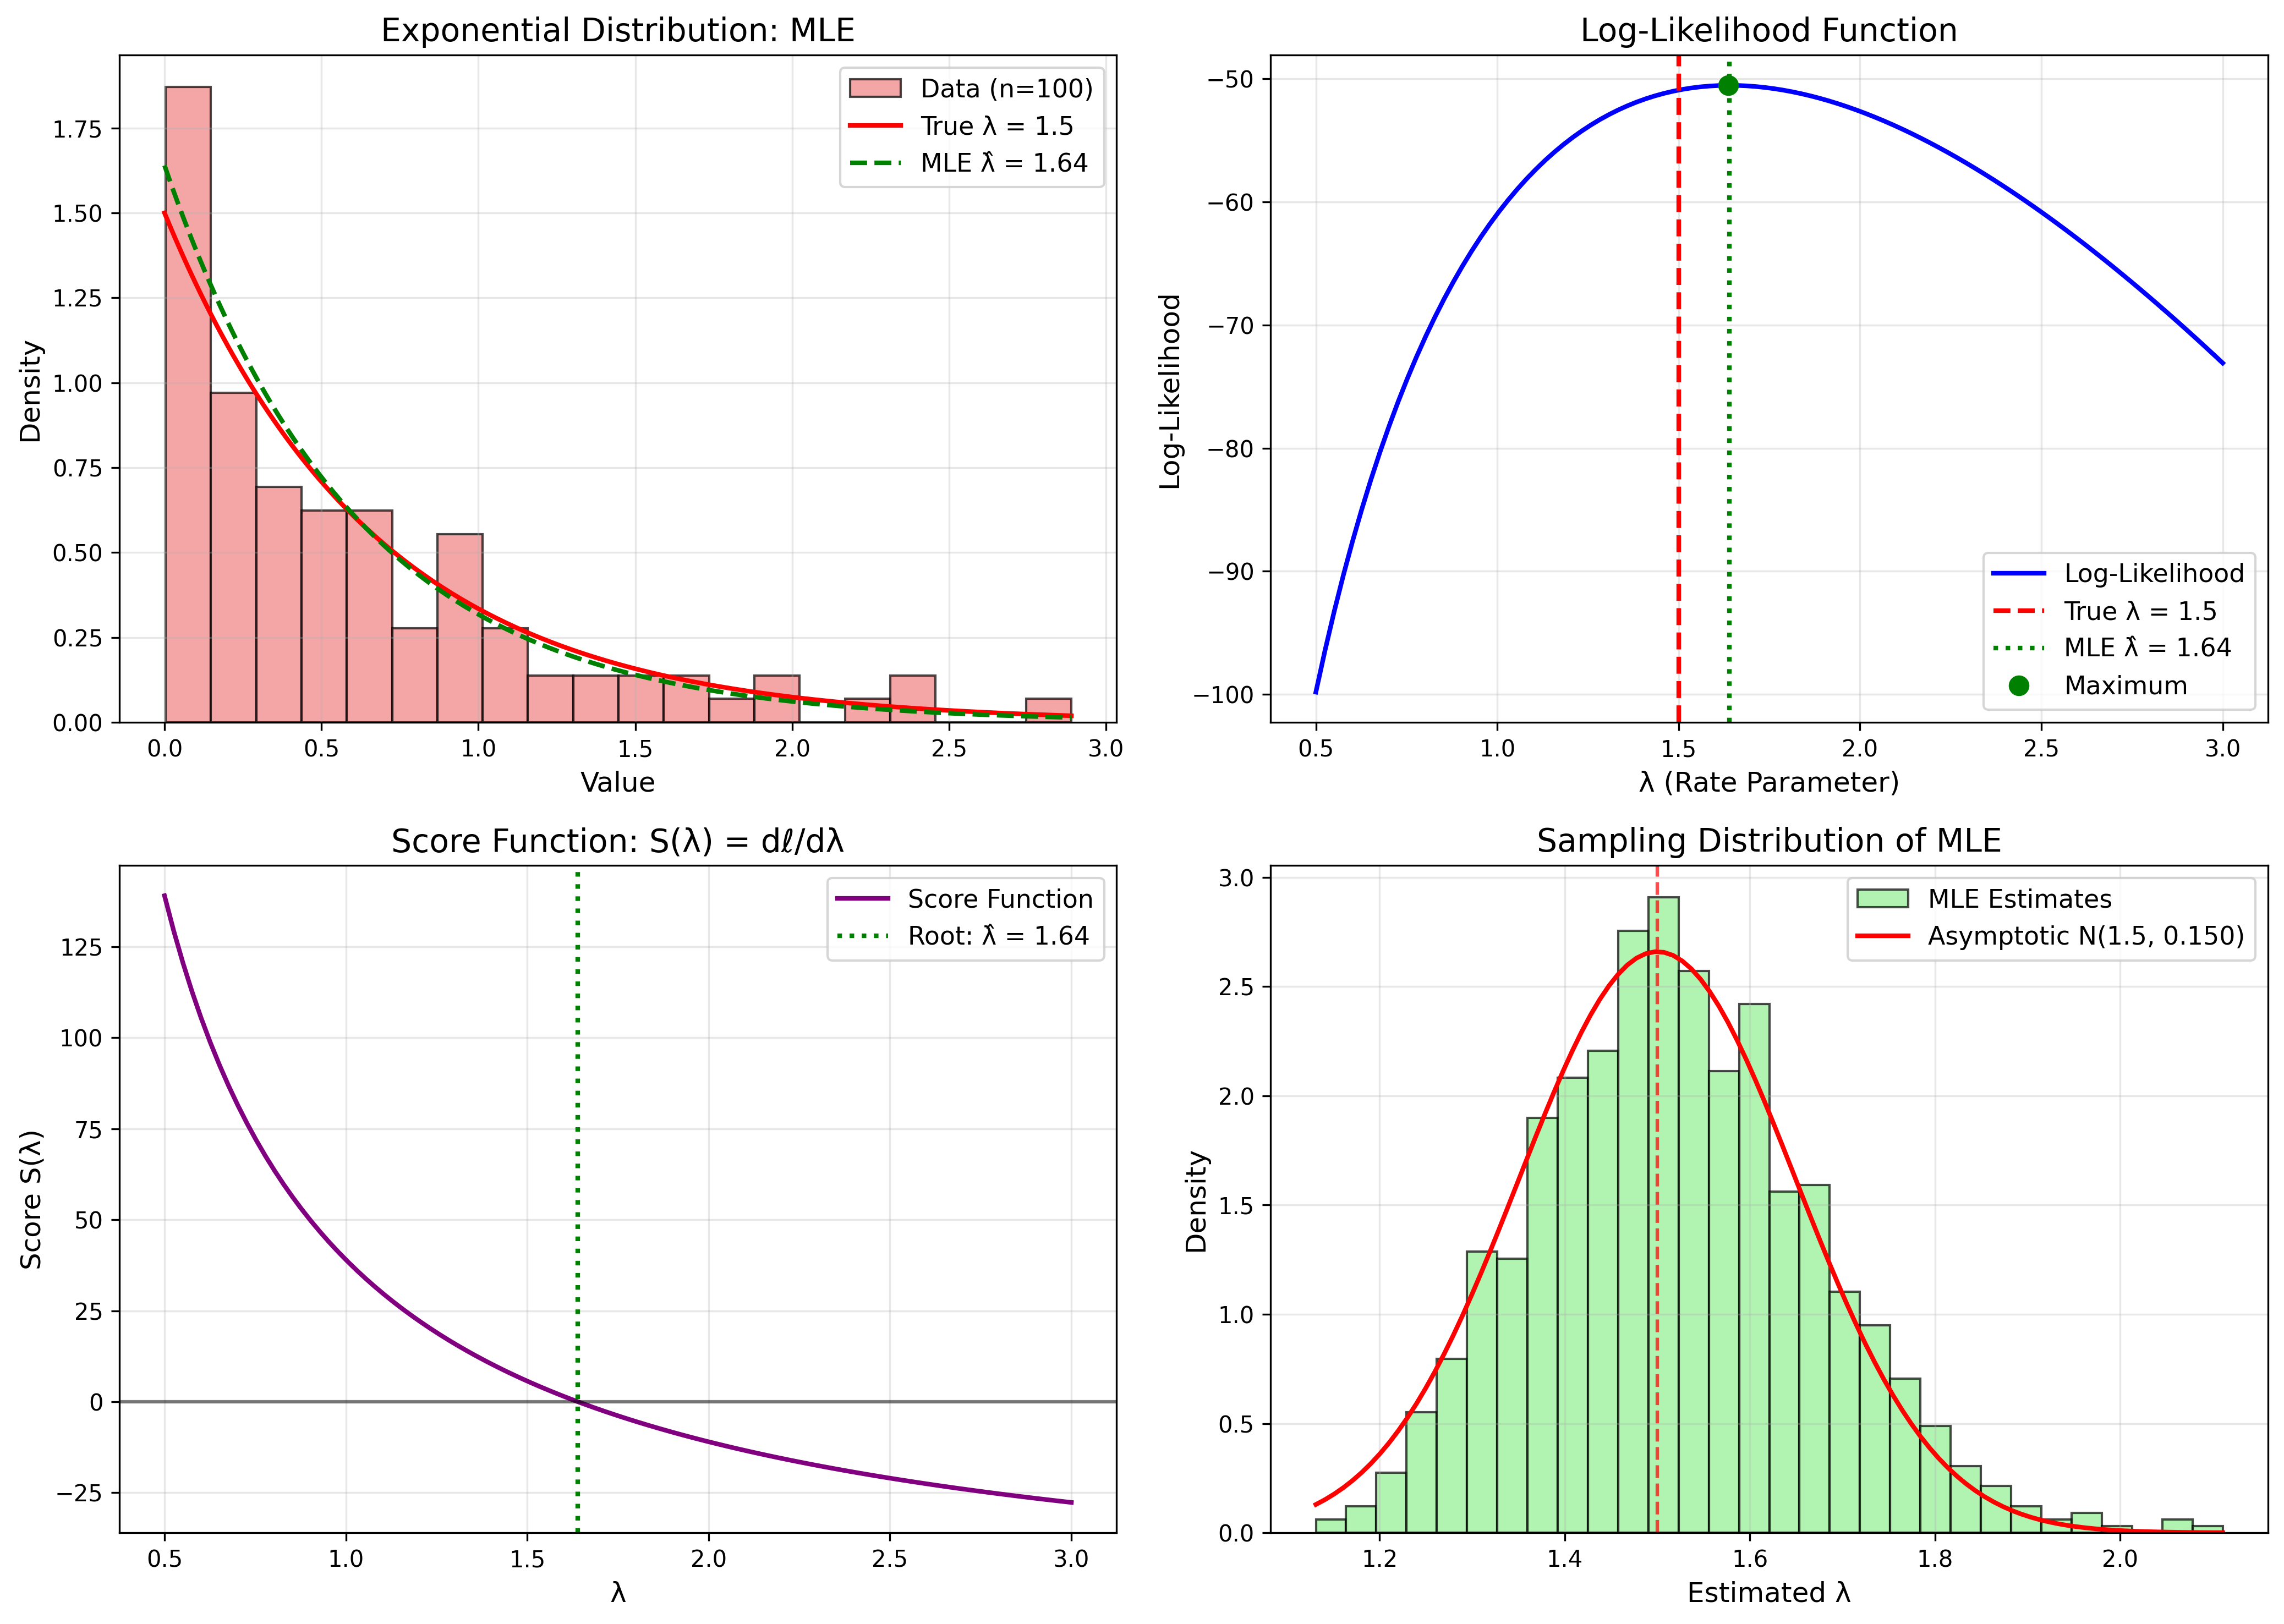
\includegraphics[width=0.6\textwidth]{../figures/mle_exponential.png}
\end{center}
\end{frame}

\begin{frame}{Properties of Maximum Likelihood Estimators}
\begin{techblock}{Asymptotic Properties (Large Sample)}
Under regularity conditions:
\begin{itemize}
\setlength{\itemsep}{1pt}
\item \textbf{Consistency:} $\hat{\theta}_{MLE} \xrightarrow{p} \theta$
\item \textbf{Asymptotic Normality:} $\sqrt{n}(\hat{\theta}_{MLE} - \theta) \xrightarrow{d} N(0, I(\theta)^{-1})$
\item \textbf{Efficiency:} Achieves Cramér-Rao lower bound
\item \textbf{Invariance:} If $\hat{\theta}$ is MLE of $\theta$, then $g(\hat{\theta})$ is MLE of $g(\theta)$
\end{itemize}
\end{techblock}


\begin{columns}[T]
\begin{column}{0.5\textwidth}
\textbf{Fisher Information:}
$$I(\theta) = -E\left[\frac{d^2\ell(\theta)}{d\theta^2}\right]$$

Higher information $\Rightarrow$ lower variance
\end{column}
\begin{column}{0.5\textwidth}
\textbf{Observed Information:}
$$J(\hat{\theta}) = -\frac{d^2\ell(\theta)}{d\theta^2}\bigg|_{\theta=\hat{\theta}}$$

Used for confidence intervals
\end{column}
\end{columns}


\begin{center}
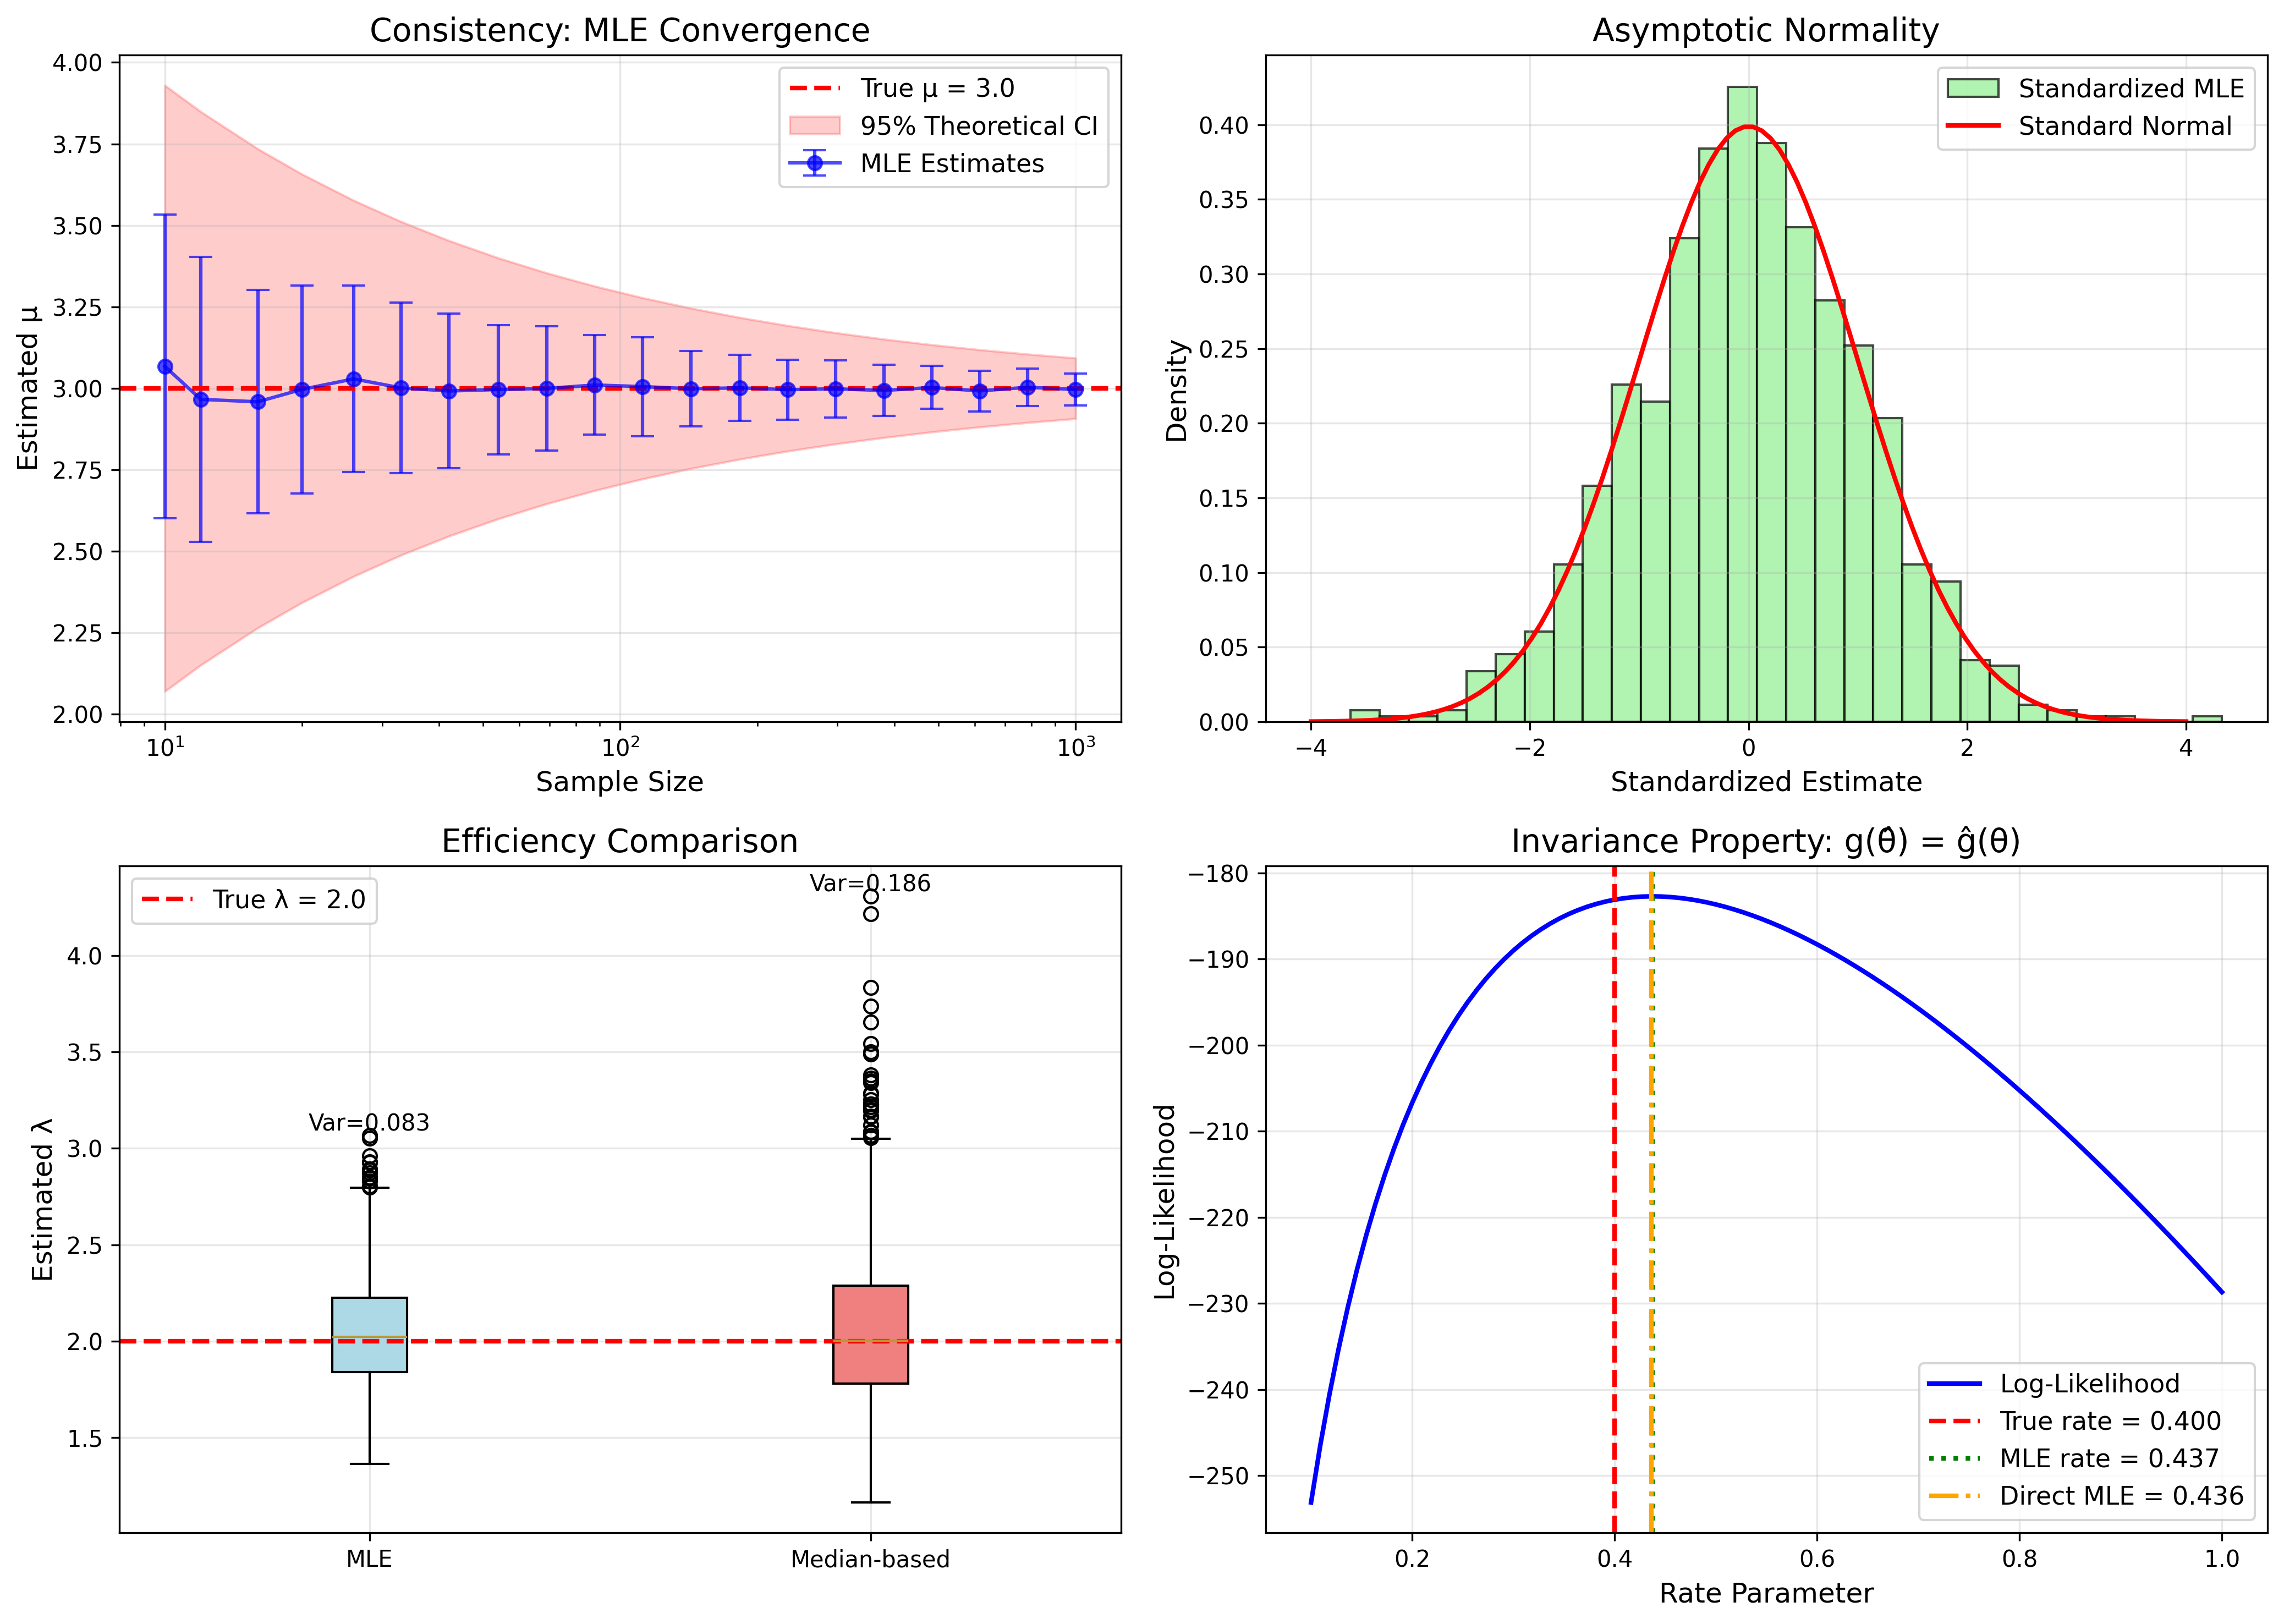
\includegraphics[width=0.6\textwidth]{../figures/mle_properties.png}
\end{center}
\end{frame}

\begin{frame}{Numerical Methods for MLE}
\begin{alertblock}{When Closed-Form Solution Doesn't Exist}
Many distributions require numerical optimization to find MLE.
\end{alertblock}


\begin{columns}[T]
\begin{column}{0.5\textwidth}
\textbf{Newton-Raphson Method:}
$$\theta^{(t+1)} = \theta^{(t)} - \frac{S(\theta^{(t)})}{J(\theta^{(t)})}$$

where $S(\theta)$ is score and $J(\theta)$ is observed information.
\end{column}
\begin{column}{0.5\textwidth}
\textbf{Other Methods:}
\begin{itemize}
\setlength{\itemsep}{1pt}
\item Gradient ascent
\item BFGS optimization
\item EM algorithm (for latent variables)
\item Grid search (for low dimensions)
\end{itemize}
\end{column}
\end{columns}


\begin{example}
For mixture of Gaussians:
$$f(x|\boldsymbol{\theta}) = \sum_{k=1}^K \pi_k N(x|\mu_k, \sigma_k^2)$$
No closed-form MLE $\Rightarrow$ Use EM algorithm
\end{example}


\begin{center}
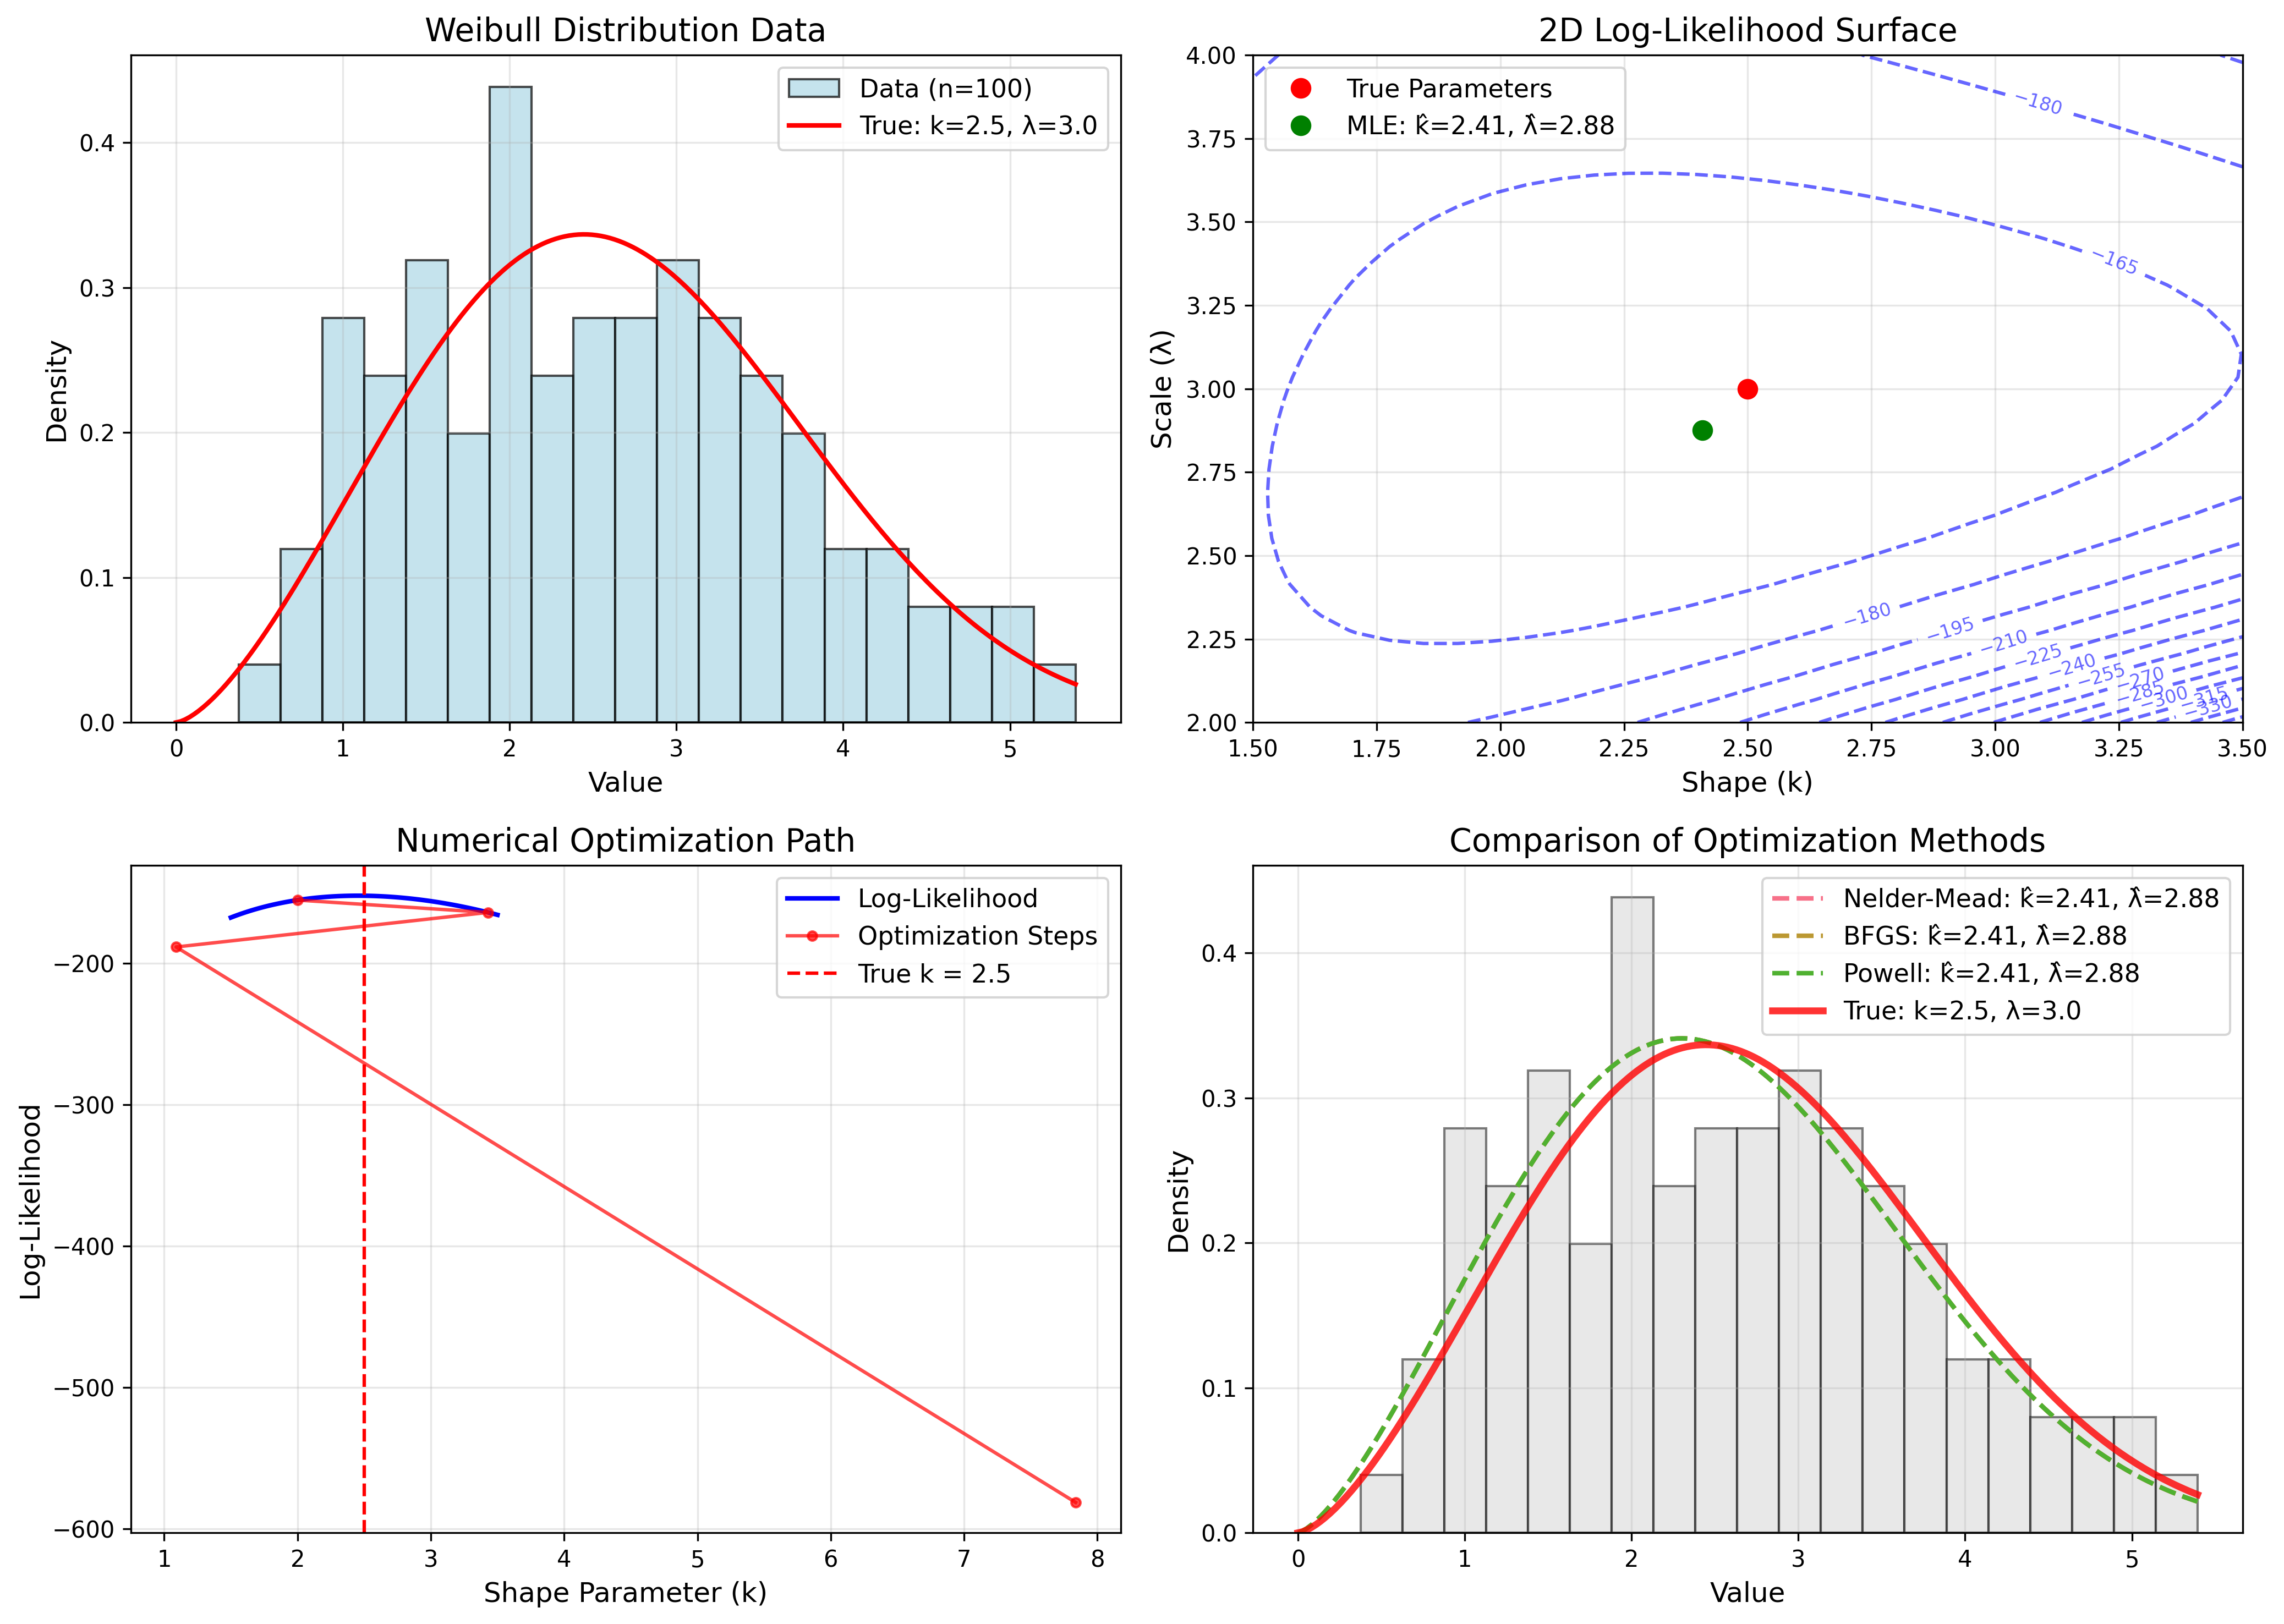
\includegraphics[width=0.6\textwidth]{../figures/numerical_mle.png}
\end{center}
\end{frame}

% SECTION 5: COMPARISON
\section{Comparison of Methods}

\begin{frame}{Method of Moments vs Maximum Likelihood}
\begin{columns}[T]
\begin{column}{0.5\textwidth}
\begin{momblock}{Method of Moments}
\textbf{Pros:}
\begin{itemize}
\setlength{\itemsep}{1pt}
\item Simple computation
\item Always exists (if moments exist)
\item Distribution-free approach
\item Good starting values for MLE
\end{itemize}

\textbf{Cons:}
\begin{itemize}
\setlength{\itemsep}{1pt}
\item Not optimal (higher variance)
\item May give invalid estimates
\item Doesn't use full data information
\end{itemize}
\end{momblock}
\end{column}
\begin{column}{0.5\textwidth}
\begin{mleblock}{Maximum Likelihood}
\textbf{Pros:}
\begin{itemize}
\setlength{\itemsep}{1pt}
\item Optimal (minimum variance)
\item Uses full data information
\item Good theoretical properties
\item Invariance property
\end{itemize}

\textbf{Cons:}
\begin{itemize}
\setlength{\itemsep}{1pt}
\item May require numerical methods
\item Can be computationally intensive
\item Requires specification of full distribution
\end{itemize}
\end{mleblock}
\end{column}
\end{columns}


\begin{center}
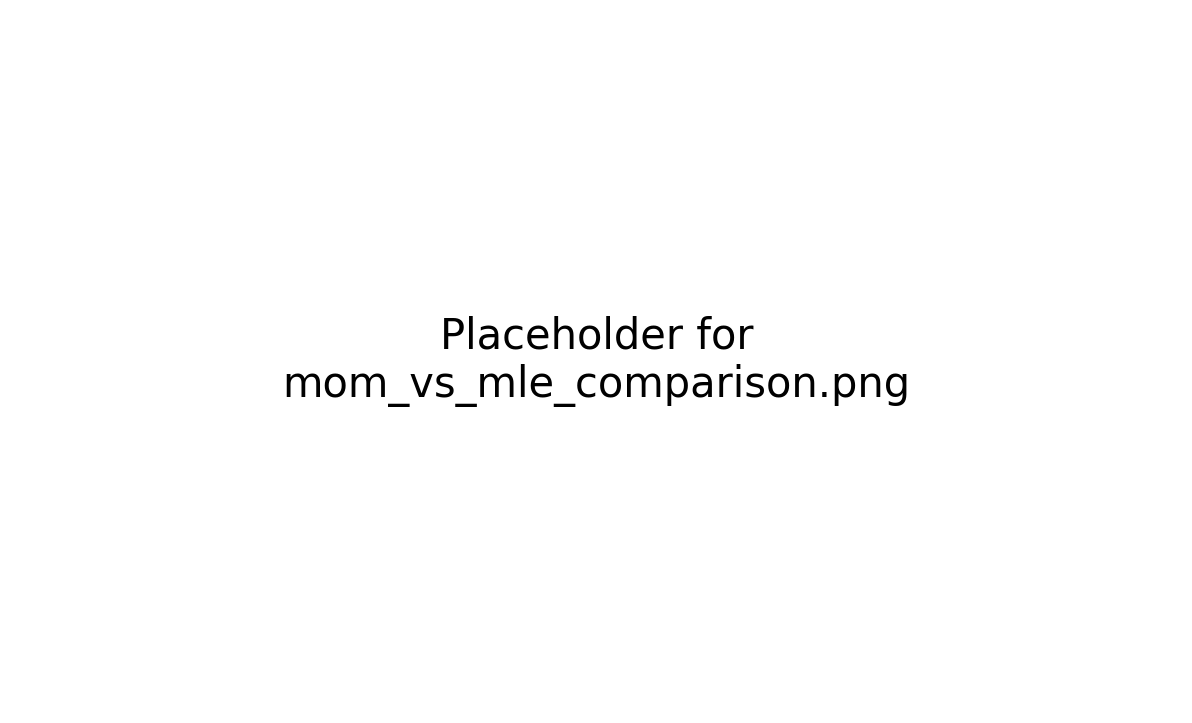
\includegraphics[width=0.6\textwidth]{../figures/mom_vs_mle_comparison.png}
\end{center}
\end{frame}

\begin{frame}{Efficiency Comparison}
\begin{techblock}{Relative Efficiency}
$$ARE = \frac{Var(\hat{\theta}_{MLE})}{Var(\hat{\theta}_{MoM})}$$
MLE is asymptotically more efficient when $ARE < 1$.
\end{techblock}


\begin{columns}[T]
\begin{column}{0.5\textwidth}
\textbf{Normal Distribution:}
\begin{itemize}
\setlength{\itemsep}{1pt}
\item For $\mu$: $ARE = 1$ (same efficiency)
\item For $\sigma^2$: $ARE = 0.5$ (MLE better)
\end{itemize}

\textbf{Exponential Distribution:}
\begin{itemize}
\setlength{\itemsep}{1pt}
\item For $\lambda$: $ARE = 1$ (same efficiency)
\end{itemize}
\end{column}
\begin{column}{0.5\textwidth}
\textbf{Gamma Distribution:}
\begin{itemize}
\setlength{\itemsep}{1pt}
\item MLE significantly more efficient
\item MoM can be quite inefficient
\end{itemize}

\textbf{General Rule:}
\begin{itemize}
\setlength{\itemsep}{1pt}
\item MLE $\geq$ MoM in efficiency
\item Difference larger for complex distributions
\end{itemize}
\end{column}
\end{columns}


\begin{center}

\includegraphics[width=0.6\textwidth]{../figures/efficiency_comparison.png}
\end{center}
\end{frame}

\begin{frame}{When to Use Which Method?}
\begin{columns}[T]
\begin{column}{0.5\textwidth}
\begin{block}{Use Method of Moments When:}
\begin{itemize}
\setlength{\itemsep}{1pt}
\item Quick estimates needed
\item Computational resources limited
\item Distribution family uncertain
\item Starting values for optimization
\item Robust estimates desired
\item Teaching/illustration purposes
\end{itemize}
\end{block}
\end{column}
\begin{column}{0.5\textwidth}
\begin{block}{Use Maximum Likelihood When:}
\begin{itemize}
\setlength{\itemsep}{1pt}
\item Optimal estimates needed
\item Distribution well-specified
\item Large sample sizes
\item Inference required (confidence intervals)
\item Model comparison needed
\item Production/research applications
\end{itemize}
\end{block}
\end{column}
\end{columns}


\begin{alertblock}{Practical Strategy}
\begin{enumerate}
\setlength{\itemsep}{1pt}
\item Start with Method of Moments for initial estimates
\item Use MoM estimates as starting values for MLE optimization
\item Compare results and choose based on application needs
\item Consider computational cost vs. statistical efficiency trade-off
\end{enumerate}
\end{alertblock}
\end{frame}

% SECTION 6: APPLICATIONS
\section{Applications}

\begin{frame}{Linear Regression Parameter Estimation}
\textbf{Model:} $y_i = \beta_0 + \beta_1 x_i + \epsilon_i$, where $\epsilon_i \sim N(0, \sigma^2)$


\begin{columns}[T]
\begin{column}{0.5\textwidth}
\textbf{Method of Moments:}
\begin{align}
E[Y] &= \beta_0 + \beta_1 E[X]\\
E[XY] &= \beta_0 E[X] + \beta_1 E[X^2]
\end{align}

Solving:
\begin{align}
\hat{\beta}_1 &= \frac{\overline{xy} - \bar{x}\bar{y}}{\overline{x^2} - \bar{x}^2}\\
\hat{\beta}_0 &= \bar{y} - \hat{\beta}_1\bar{x}
\end{align}
\end{column}
\begin{column}{0.5\textwidth}
\textbf{Maximum Likelihood:}
\begin{align}
\ell(\boldsymbol{\beta}, \sigma^2) = -\frac{n}{2}\log(2\pi\sigma^2) - \frac{1}{2\sigma^2}\sum_{i=1}^n (y_i - \beta_0 - \beta_1 x_i)^2
\end{align}

MLE gives same result:
\begin{align}
\hat{\beta}_1 &= \frac{\sum(x_i - \bar{x})(y_i - \bar{y})}{\sum(x_i - \bar{x})^2}\\
\hat{\beta}_0 &= \bar{y} - \hat{\beta}_1\bar{x}
\end{align}
\end{column}
\end{columns}


\begin{center}
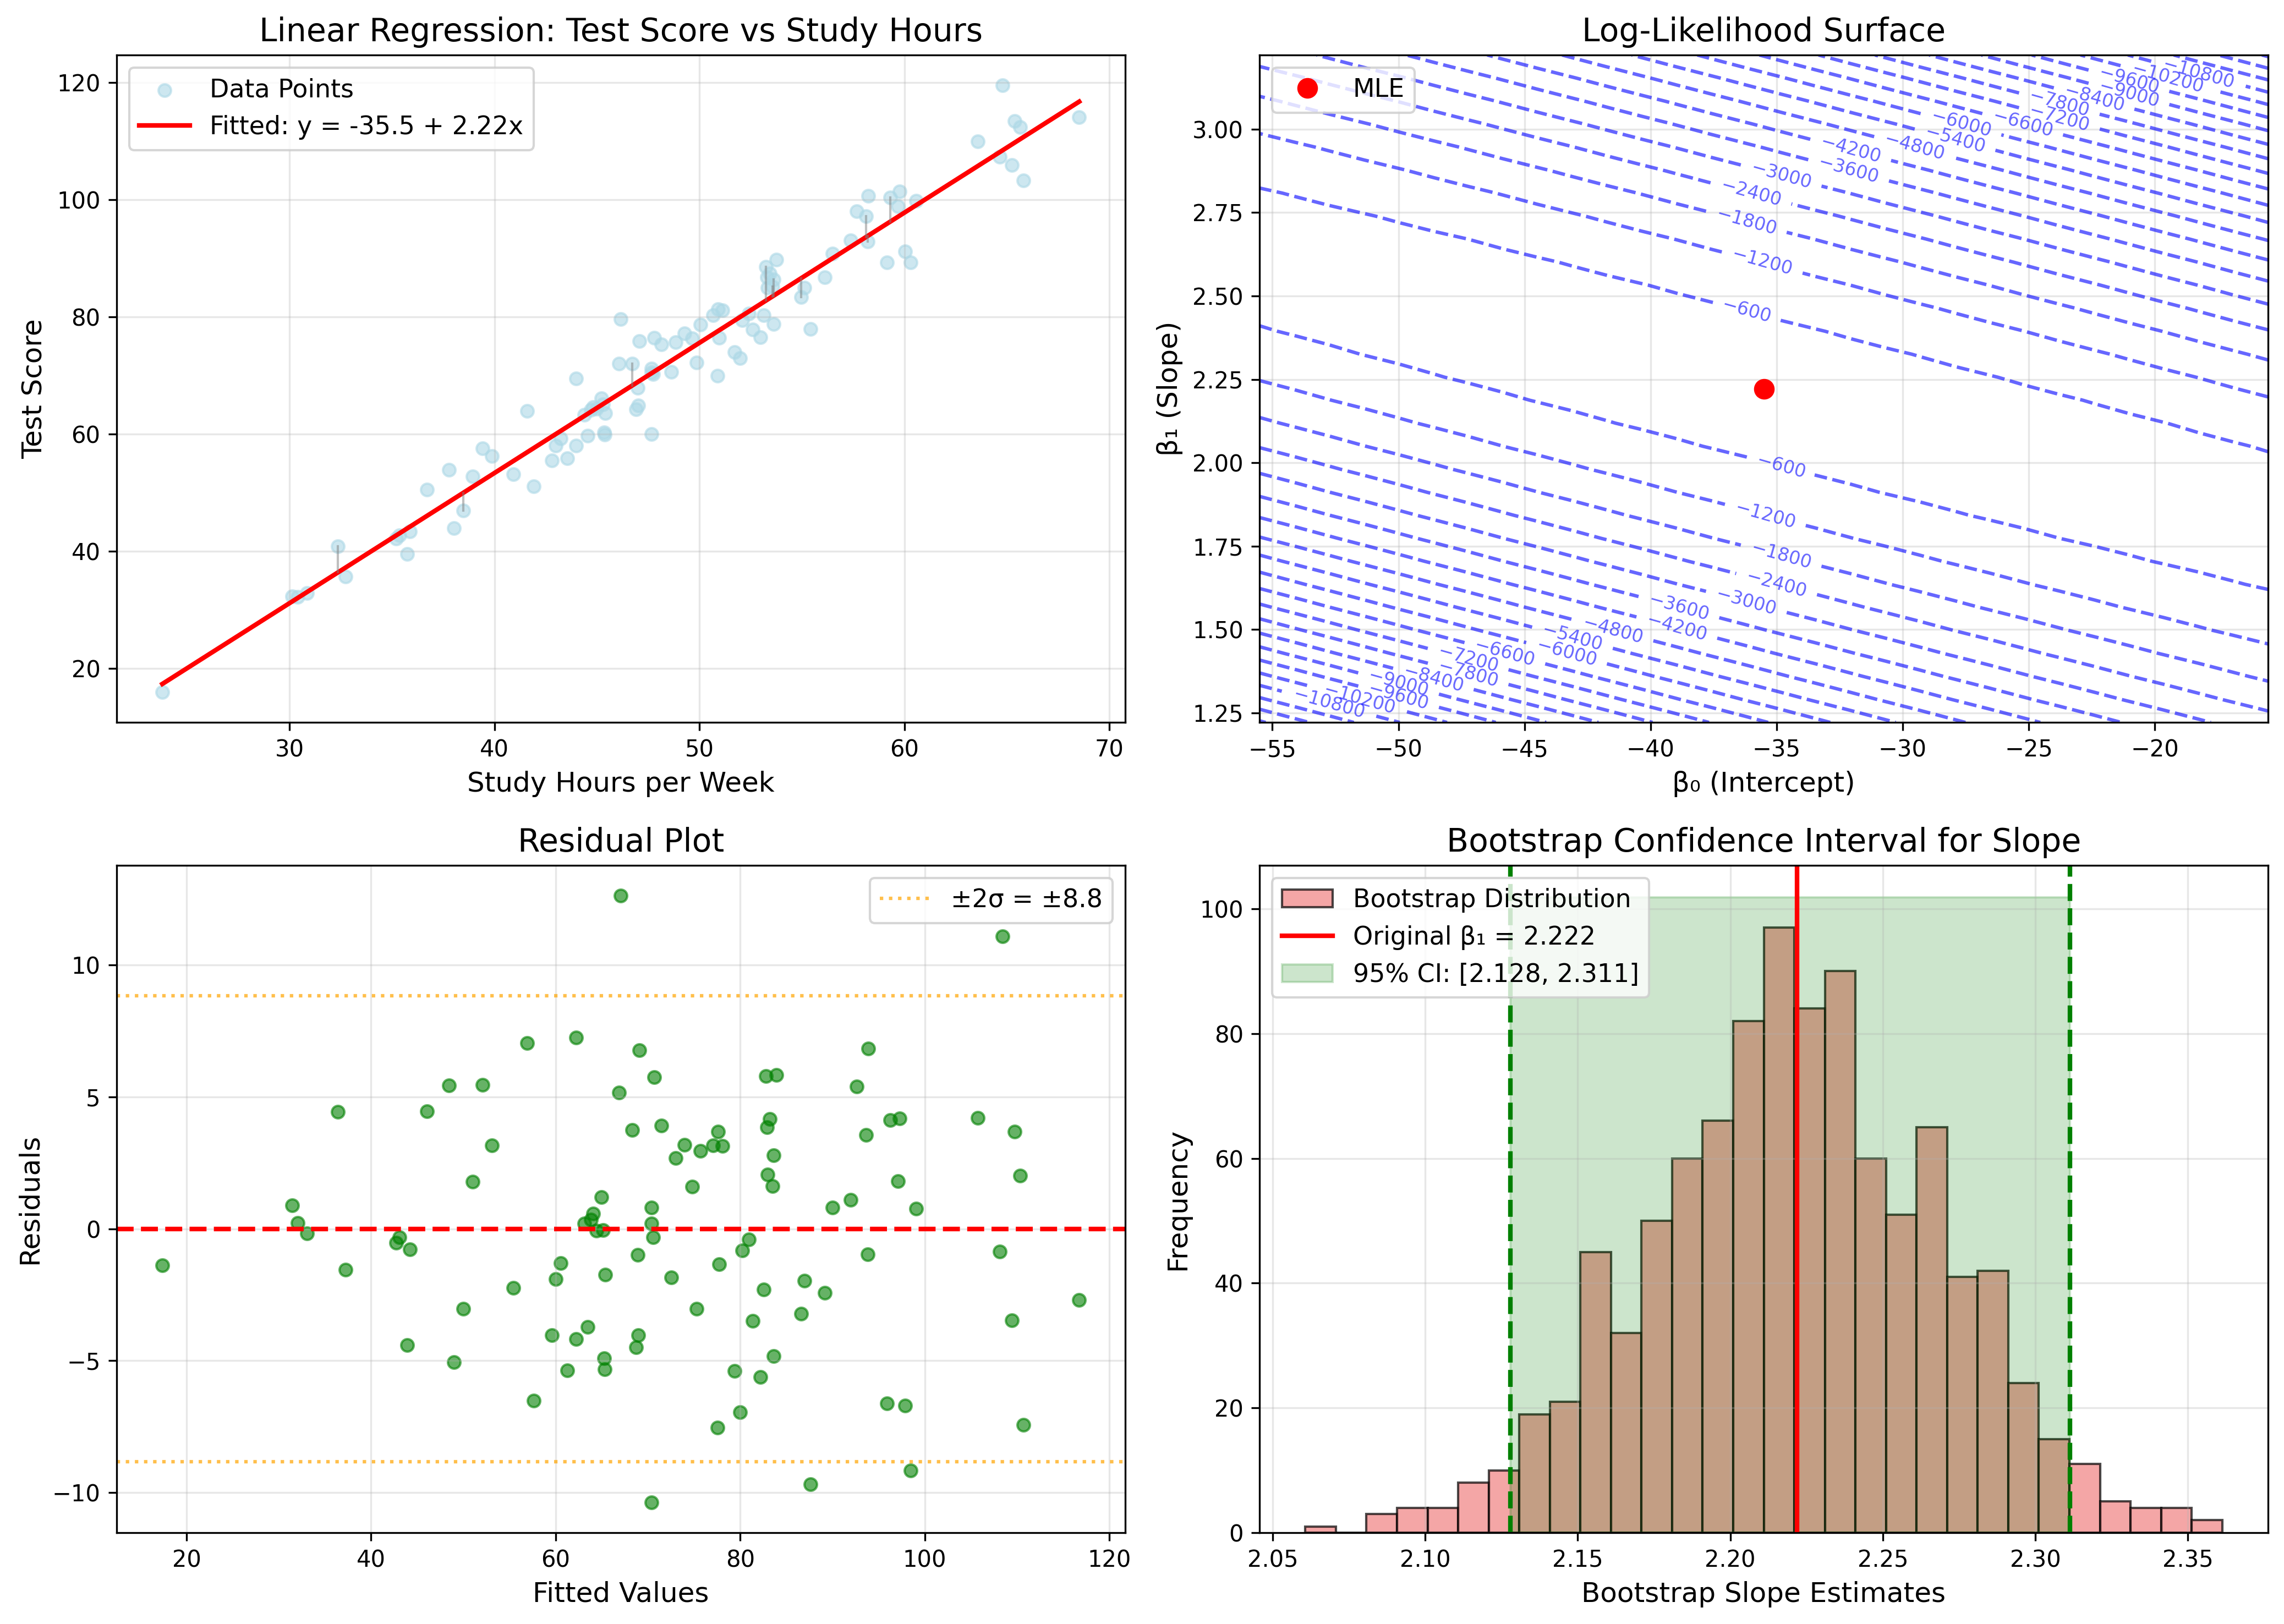
\includegraphics[width=0.6\textwidth]{../figures/linear_regression_estimation.png}
\end{center}
\end{frame}

\begin{frame}{Logistic Regression Parameter Estimation}
\textbf{Model:} $P(Y=1|X) = \frac{1}{1 + e^{-(\beta_0 + \beta_1 X)}}$


\begin{alertblock}{No Closed-Form Solution}
Logistic regression requires numerical optimization for MLE.
\end{alertblock}

\textbf{Log-likelihood:}
$$\ell(\boldsymbol{\beta}) = \sum_{i=1}^n \left[y_i(\beta_0 + \beta_1 x_i) - \log(1 + e^{\beta_0 + \beta_1 x_i})\right]$$

\textbf{Score equations:}
\begin{align}
\frac{\partial \ell}{\partial \beta_0} &= \sum_{i=1}^n (y_i - p_i) = 0\\
\frac{\partial \ell}{\partial \beta_1} &= \sum_{i=1}^n x_i(y_i - p_i) = 0
\end{align}

where $p_i = \frac{1}{1 + e^{-(\beta_0 + \beta_1 x_i)}}$


\begin{center}
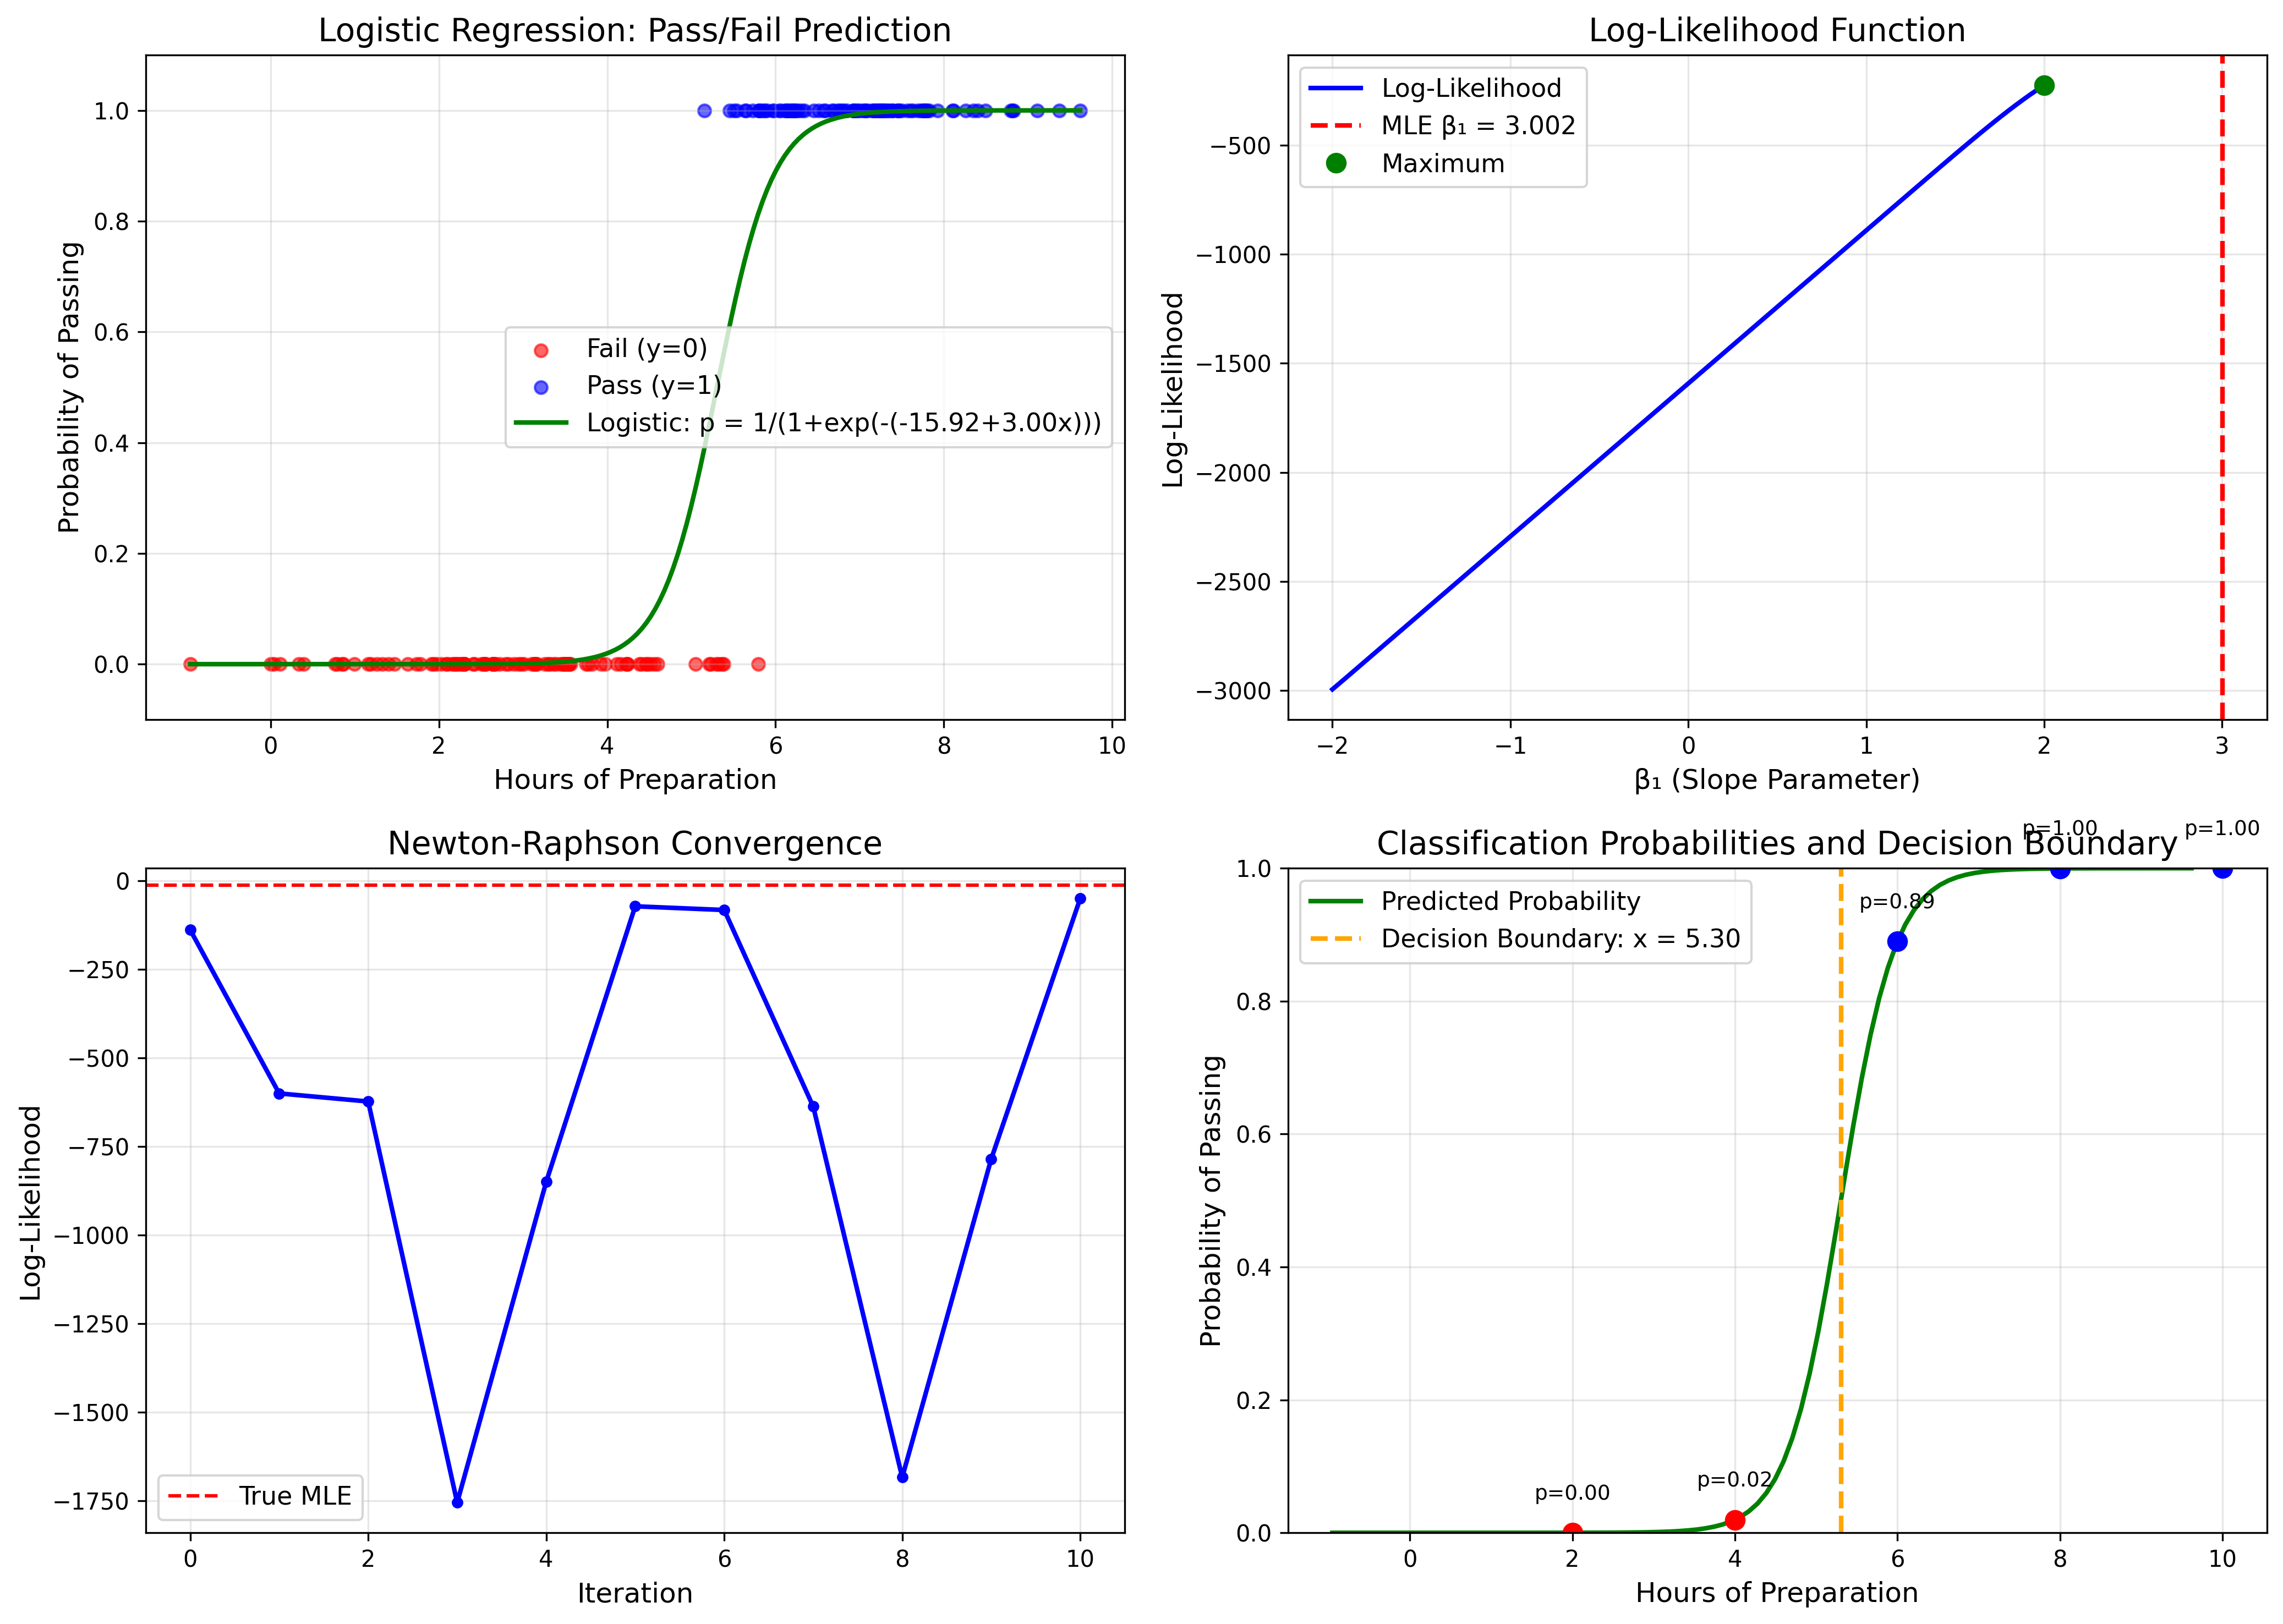
\includegraphics[width=0.6\textwidth]{../figures/logistic_regression_estimation.png}
\end{center}
\end{frame}

\begin{frame}{Clustering: Gaussian Mixture Models}
\textbf{Model:} $f(x|\boldsymbol{\theta}) = \sum_{k=1}^K \pi_k N(x|\mu_k, \sigma_k^2)$


\begin{columns}[T]
\begin{column}{0.5\textwidth}
\textbf{Parameters to estimate:}
\begin{itemize}
\setlength{\itemsep}{1pt}
\item Mixing weights: $\pi_1, \ldots, \pi_K$
\item Means: $\mu_1, \ldots, \mu_K$
\item Variances: $\sigma_1^2, \ldots, \sigma_K^2$
\end{itemize}
\end{column}
\begin{column}{0.5\textwidth}
\textbf{Challenges:}
\begin{itemize}
\setlength{\itemsep}{1pt}
\item Latent variables (cluster assignments)
\item Complex likelihood surface
\item Local optima
\item Model selection (choosing $K$)
\end{itemize}
\end{column}
\end{columns}


\begin{techblock}{EM Algorithm}
\textbf{E-step:} Compute posterior probabilities of cluster assignments\\
\textbf{M-step:} Update parameters using weighted MLE
\end{techblock}


\begin{center}
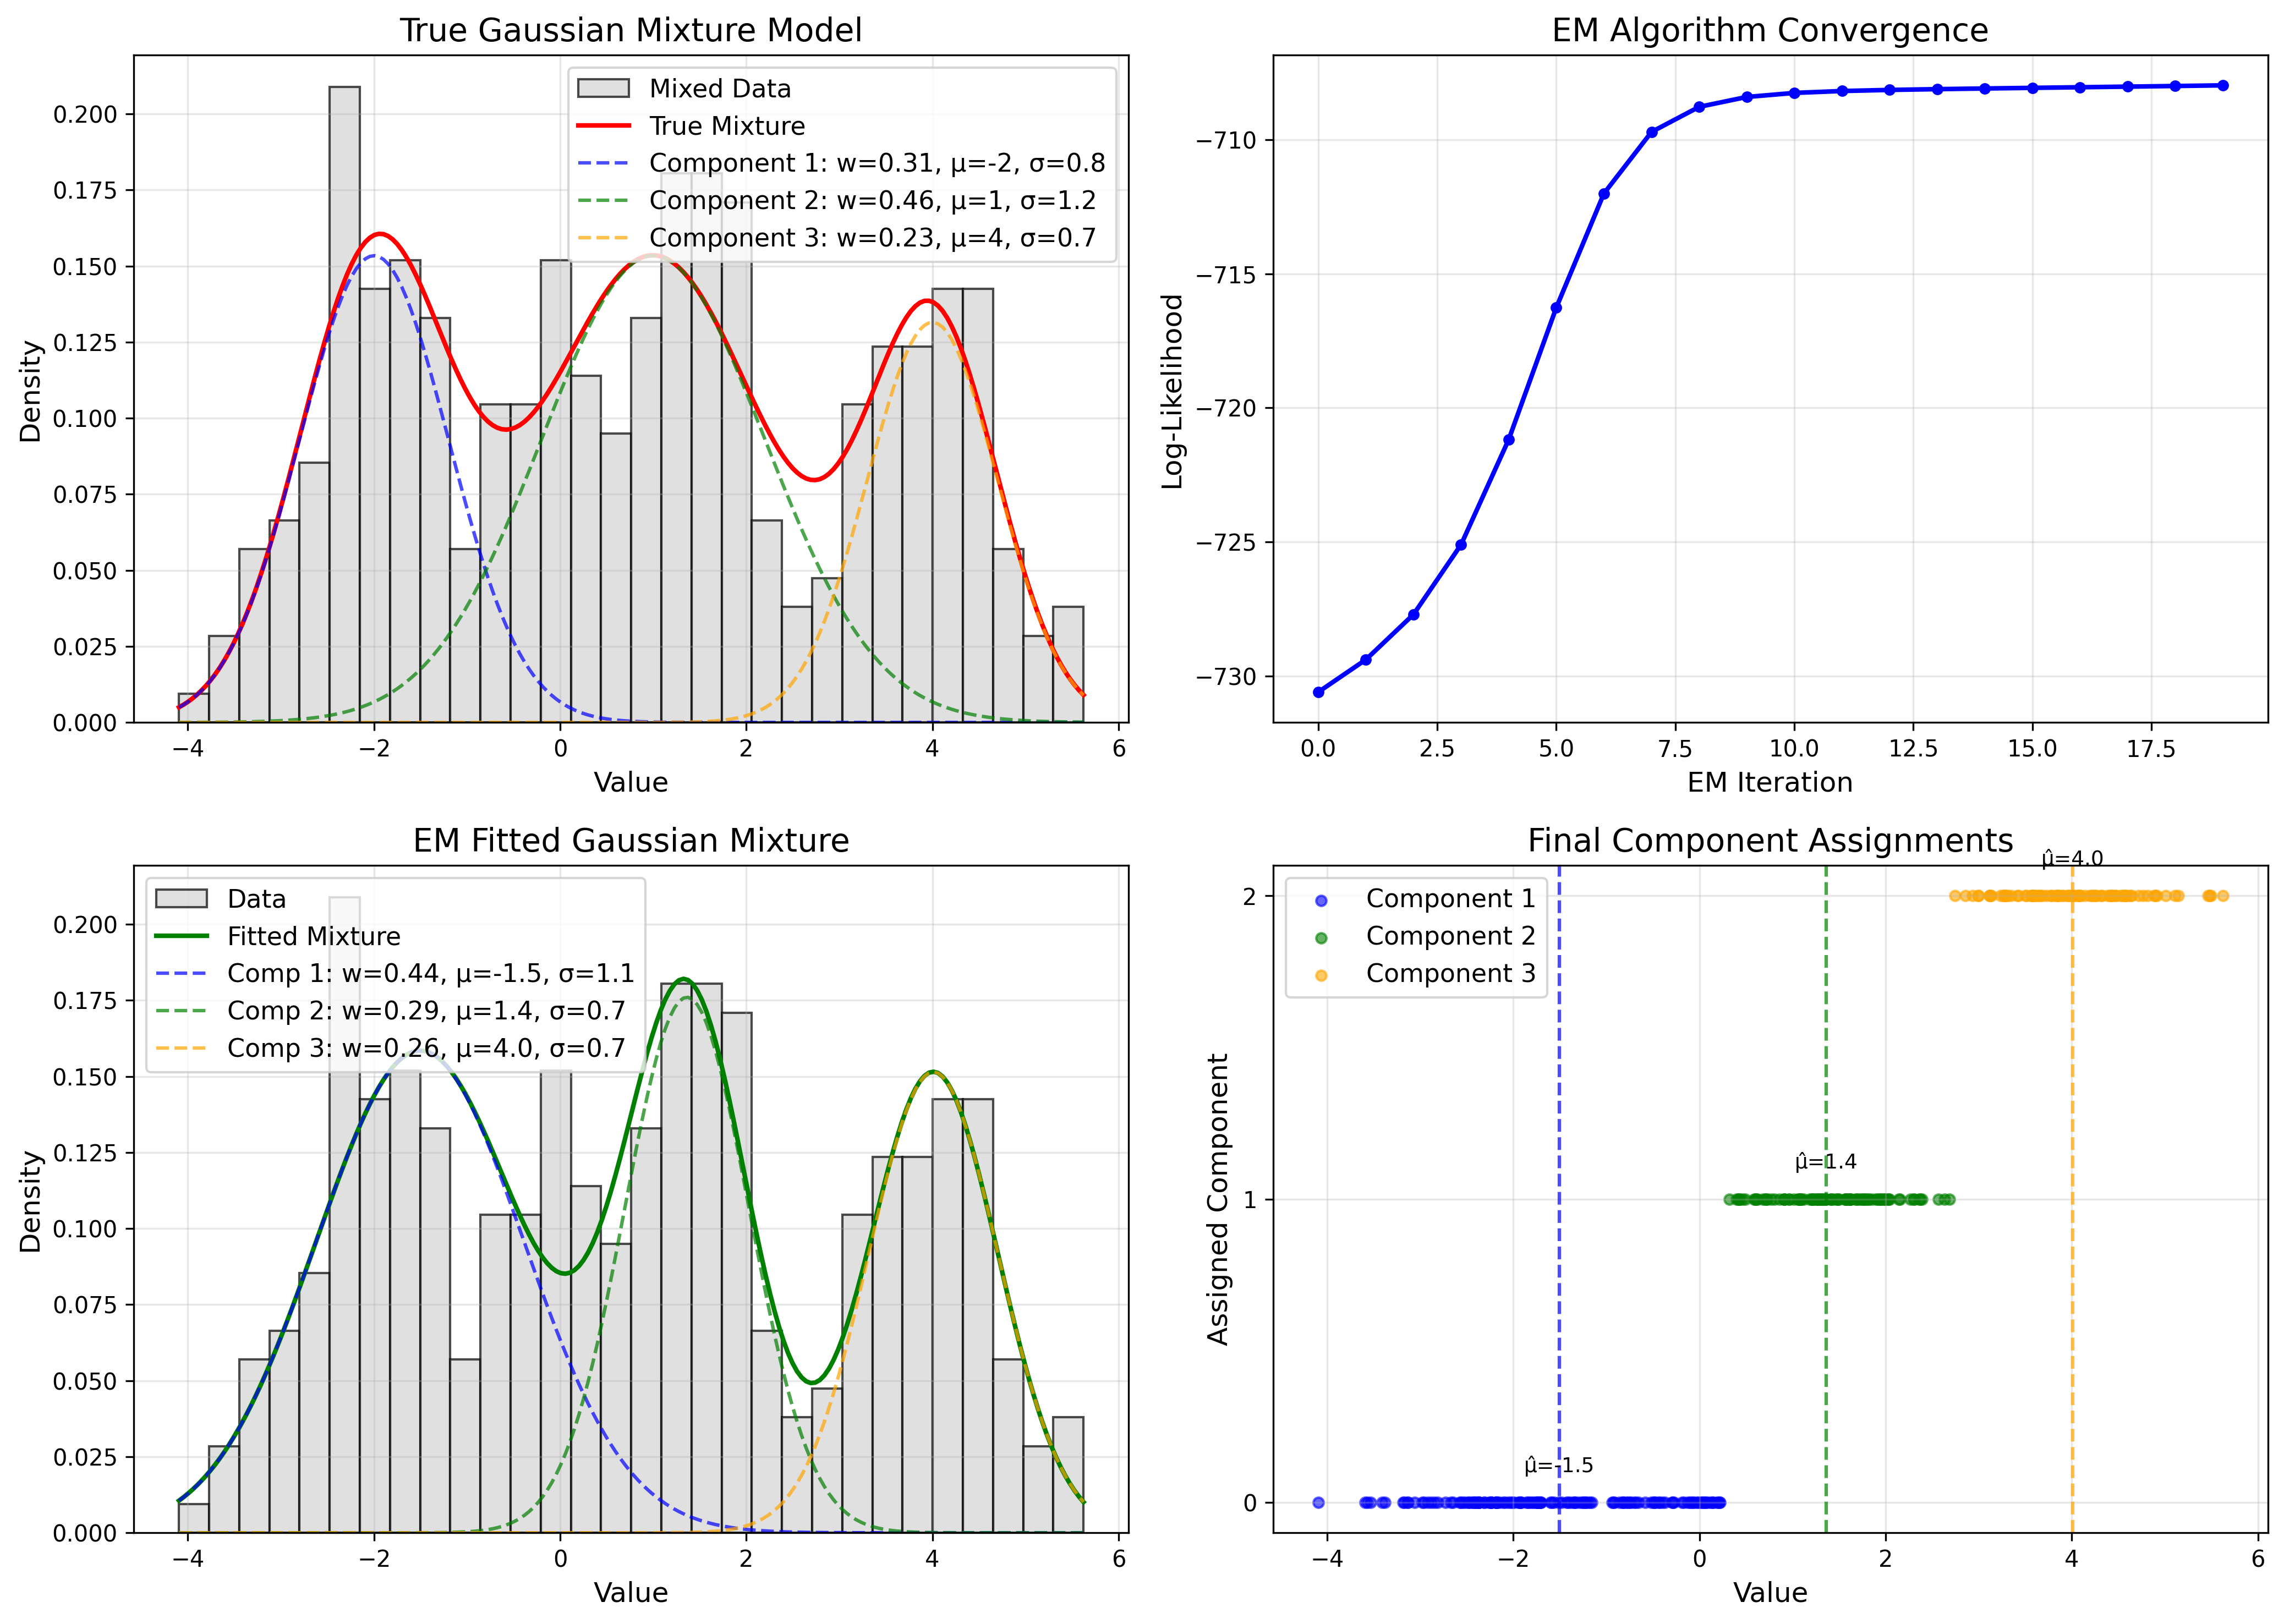
\includegraphics[width=0.6\textwidth]{../figures/gaussian_mixture_estimation.png}
\end{center}
\end{frame}

\begin{frame}{Time Series: ARIMA Parameters}
\textbf{ARIMA(p,d,q) Model:}
$$(1-\phi_1B-\cdots-\phi_pB^p)(1-B)^d X_t = (1+\theta_1B+\cdots+\theta_qB^q)\epsilon_t$$


\begin{columns}[T]
\begin{column}{0.5\textwidth}
\textbf{Method of Moments:}
\begin{itemize}
\setlength{\itemsep}{1pt}
\item Use sample autocorrelations
\item Yule-Walker equations for AR parts
\item Moment conditions for MA parts
\item Simple but not optimal
\end{itemize}
\end{column}
\begin{column}{0.5\textwidth}
\textbf{Maximum Likelihood:}
\begin{itemize}
\setlength{\itemsep}{1pt}
\item Kalman filter for likelihood
\item Numerical optimization required
\item More efficient estimates
\item Standard errors available
\end{itemize}
\end{column}
\end{columns}


\begin{example}
AR(1): $X_t = \phi X_{t-1} + \epsilon_t$
\begin{itemize}
\setlength{\itemsep}{1pt}
\item MoM: $\hat{\phi} = \hat{\rho}_1$ (sample autocorrelation)
\item MLE: Optimize $\ell(\phi, \sigma^2)$ numerically
\end{itemize}
\end{example}


\begin{center}
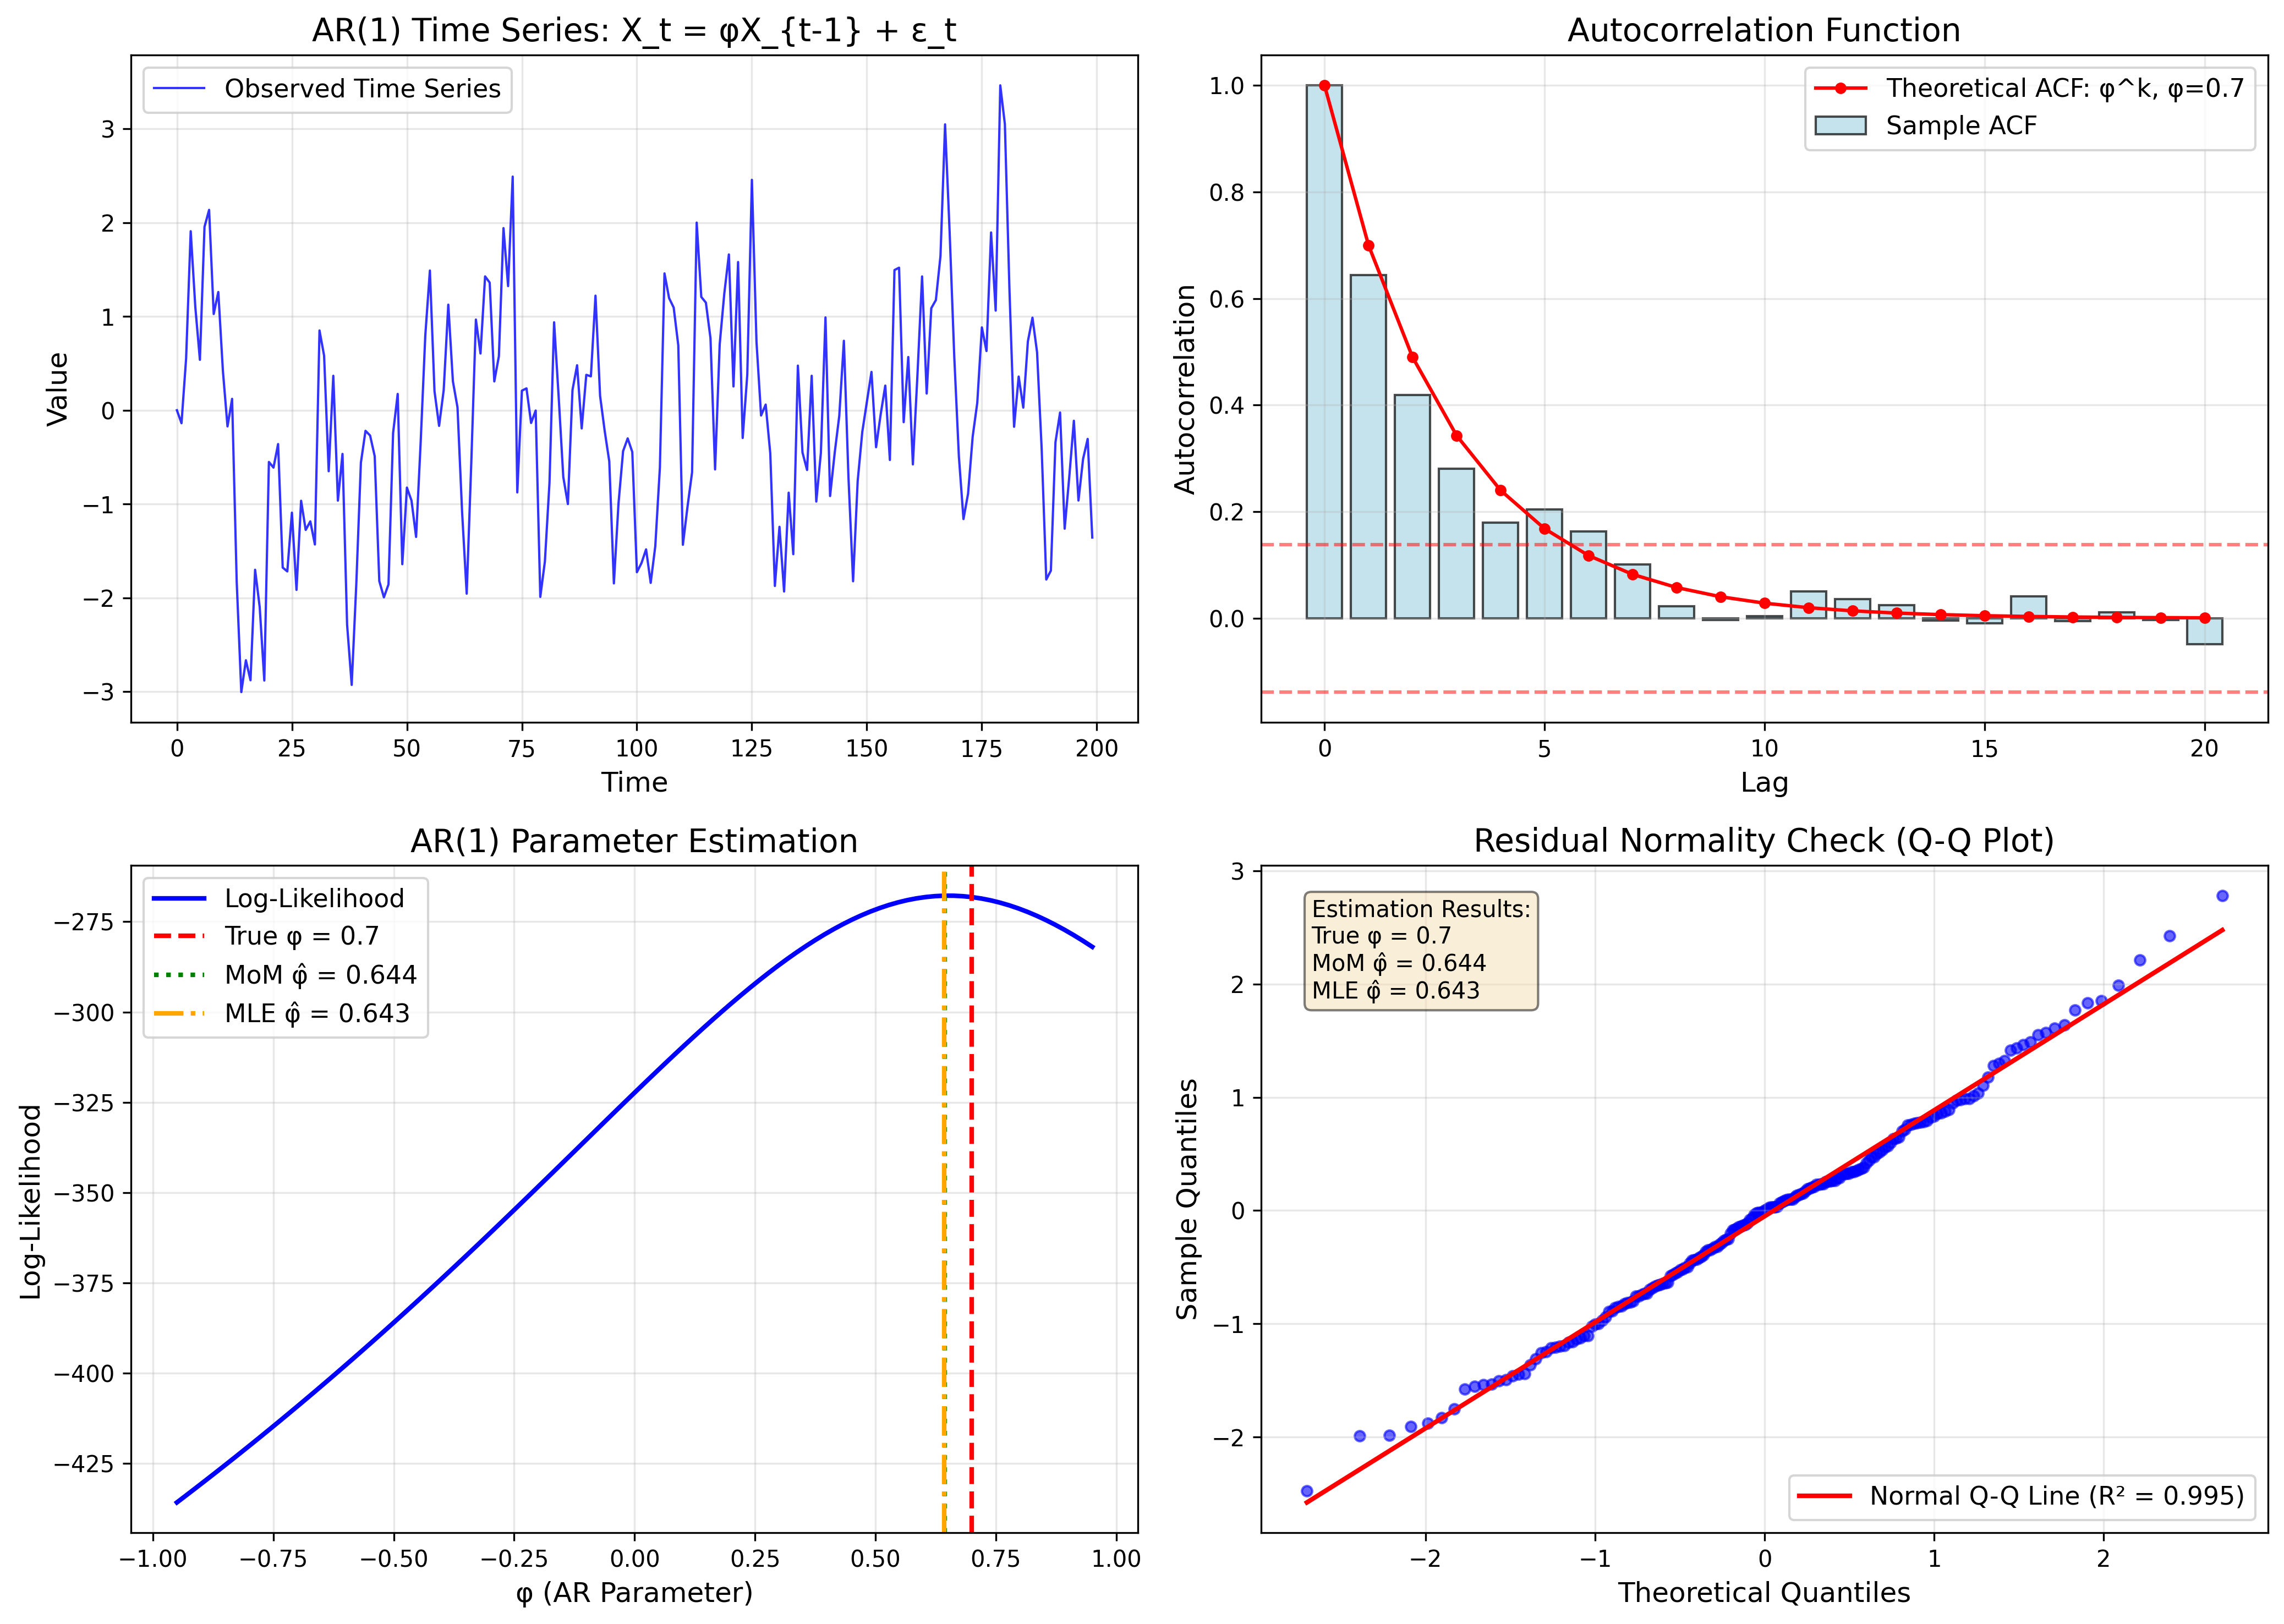
\includegraphics[width=0.6\textwidth]{../figures/arima_estimation.png}
\end{center}
\end{frame}

% SECTION 7: ADVANCED TOPICS
\section{Advanced Topics}

\begin{frame}{Bayesian Parameter Estimation}
\begin{techblock}{Bayesian Approach}
Treat parameters as random variables with prior distributions.
\end{techblock}

\textbf{Bayes' Theorem:}
$$p(\theta|x) = \frac{p(x|\theta)p(\theta)}{p(x)} \propto p(x|\theta)p(\theta)$$


\begin{columns}[T]
\begin{column}{0.5\textwidth}
\textbf{Components:}
\begin{itemize}
\setlength{\itemsep}{1pt}
\item $p(\theta)$: Prior distribution
\item $p(x|\theta)$: Likelihood
\item $p(\theta|x)$: Posterior distribution
\item $p(x)$: Marginal likelihood
\end{itemize}
\end{column}
\begin{column}{0.5\textwidth}
\textbf{Estimation:}
\begin{itemize}
\setlength{\itemsep}{1pt}
\item MAP: $\hat{\theta}_{MAP} = \arg\max p(\theta|x)$
\item Posterior mean: $\hat{\theta}_{PM} = E[\theta|x]$
\item Credible intervals available
\end{itemize}
\end{column}
\end{columns}


\begin{example}
Normal with normal prior:
Prior: $\mu \sim N(\mu_0, \tau^2)$, Likelihood: $X|\mu \sim N(\mu, \sigma^2)$
Posterior: $\mu|x \sim N\left(\frac{\tau^2 \bar{x} + \sigma^2\mu_0/n}{\tau^2 + \sigma^2/n}, \frac{\tau^2\sigma^2/n}{\tau^2 + \sigma^2/n}\right)$
\end{example}
\end{frame}

\begin{frame}{Robust Parameter Estimation}
\begin{alertblock}{Problem with MLE}
MLE can be sensitive to outliers and model misspecification.
\end{alertblock}


\begin{columns}[T]
\begin{column}{0.5\textwidth}
\textbf{Robust Alternatives:}
\begin{itemize}
\setlength{\itemsep}{1pt}
\item \textbf{M-estimators:} Generalize MLE
\item \textbf{Huber estimator:} Robust to outliers
\item \textbf{Trimmed means:} Remove extreme values
\item \textbf{Median-based:} Use median instead of mean
\end{itemize}
\end{column}
\begin{column}{0.5\textwidth}
\textbf{Example - Huber Loss:}
$$\rho(x) = \begin{cases}
\frac{1}{2}x^2 & |x| \leq k\\
k|x| - \frac{1}{2}k^2 & |x| > k
\end{cases}$$

Quadratic for small errors, linear for large errors.
\end{column}
\end{columns}


\begin{techblock}{Trade-offs}
Robust methods sacrifice some efficiency for stability against outliers.
\end{techblock}


\begin{center}
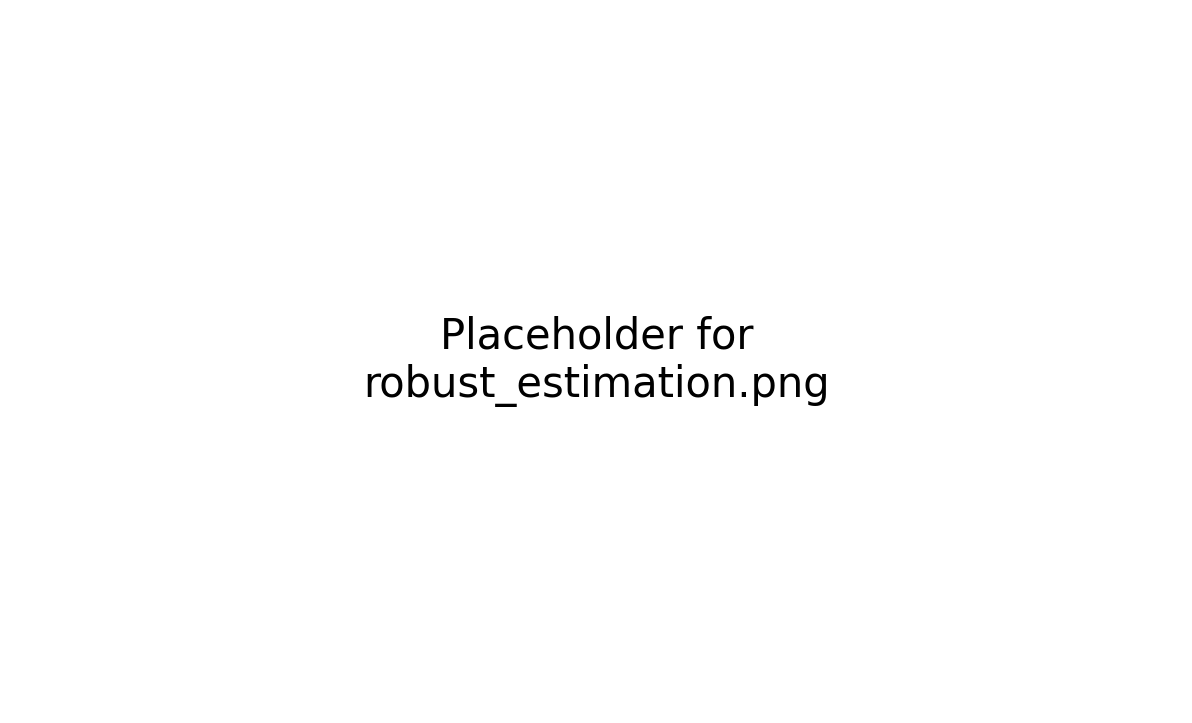
\includegraphics[width=0.6\textwidth]{../figures/robust_estimation.png}
\end{center}
\end{frame}

\begin{frame}{Bootstrap and Resampling}
\begin{techblock}{Bootstrap Principle}
Estimate sampling distribution by resampling from the observed data.
\end{techblock}

\textbf{Algorithm:}
\begin{enumerate}
\setlength{\itemsep}{1pt}
\item Draw $B$ bootstrap samples: $\{x_1^*, \ldots, x_n^*\}$ from original data
\item Compute estimate for each sample: $\hat{\theta}_b^*$
\item Use distribution of $\{\hat{\theta}_1^*, \ldots, \hat{\theta}_B^*\}$ for inference
\end{enumerate}


\begin{columns}[T]
\begin{column}{0.5\textwidth}
\textbf{Applications:}
\begin{itemize}
\setlength{\itemsep}{1pt}
\item Confidence intervals
\item Bias correction
\item Variance estimation
\item Hypothesis testing
\end{itemize}
\end{column}
\begin{column}{0.5\textwidth}
\textbf{Bootstrap Confidence Interval:}
For 95% CI, use 2.5th and 97.5th percentiles of $\{\hat{\theta}_b^*\}$.

\textbf{Bias Correction:}
$$\hat{\theta}_{corrected} = 2\hat{\theta} - \bar{\theta}^*$$
\end{column}
\end{columns}


\begin{center}
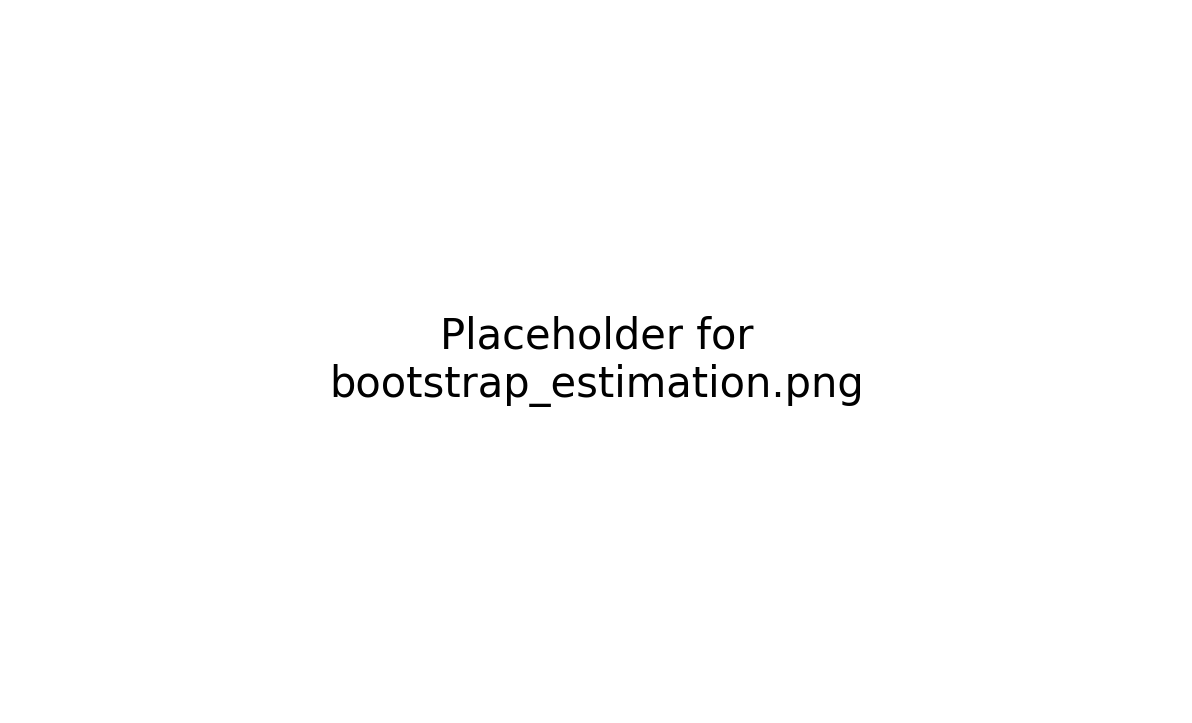
\includegraphics[width=0.6\textwidth]{../figures/bootstrap_estimation.png}
\end{center}
\end{frame}

\begin{frame}{Model Selection and Information Criteria}
\begin{techblock}{Model Selection Problem}
How do we choose between different models or number of parameters?
\end{techblock}

\textbf{Information Criteria:}
\begin{align}
AIC &= -2\ell(\hat{\theta}) + 2k\\
BIC &= -2\ell(\hat{\theta}) + k\log n\\
AICc &= AIC + \frac{2k(k+1)}{n-k-1}
\end{align}

where $k$ = number of parameters, $n$ = sample size.


\begin{columns}[T]
\begin{column}{0.5\textwidth}
\textbf{Interpretation:}
\begin{itemize}
\setlength{\itemsep}{1pt}
\item Lower values = better models
\item Trade-off: fit vs complexity
\item AIC: prediction focus
\item BIC: true model focus
\end{itemize}
\end{column}
\begin{column}{0.5\textwidth}
\textbf{Cross-Validation:}
\begin{itemize}
\setlength{\itemsep}{1pt}
\item Split data into train/validation
\item Estimate on training set
\item Evaluate on validation set
\item Choose model with best CV score
\end{itemize}
\end{column}
\end{columns}


\begin{center}

\includegraphics[width=0.6\textwidth]{../figures/model_selection.png}
\end{center}
\end{frame}

% SECTION 8: BEST PRACTICES
\section{Best Practices}

\begin{frame}{Common Pitfalls and How to Avoid Them}
\begin{columns}[T]
\begin{column}{0.5\textwidth}
\begin{alertblock}{Pitfall 1: Wrong Distribution}
Assuming incorrect distributional family leads to biased estimates.

\textbf{Solution:}
\begin{itemize}
\setlength{\itemsep}{1pt}
\item Exploratory data analysis
\item Goodness-of-fit tests
\item Residual analysis
\item Model comparison
\end{itemize}
\end{alertblock}
\end{column}
\begin{column}{0.5\textwidth}
\begin{alertblock}{Pitfall 2: Insufficient Data}
Small samples lead to unreliable estimates.

\textbf{Solution:}
\begin{itemize}
\setlength{\itemsep}{1pt}
\item Check sample size requirements
\item Use bootstrap for uncertainty
\item Consider Bayesian methods
\item Regularization techniques
\end{itemize}
\end{alertblock}
\end{column}
\end{columns}


\begin{columns}[T]
\begin{column}{0.5\textwidth}
\begin{alertblock}{Pitfall 3: Outliers}
Extreme values can severely affect estimates.

\textbf{Solution:}
\begin{itemize}
\setlength{\itemsep}{1pt}
\item Data visualization
\item Robust estimation methods
\item Outlier detection and treatment
\item Sensitivity analysis
\end{itemize}
\end{alertblock}
\end{column}
\begin{column}{0.5\textwidth}
\begin{alertblock}{Pitfall 4: Overfitting}
Too many parameters relative to data.

\textbf{Solution:}
\begin{itemize}
\setlength{\itemsep}{1pt}
\item Information criteria (AIC, BIC)
\item Cross-validation
\item Regularization (Ridge, Lasso)
\item Domain knowledge constraints
\end{itemize}
\end{alertblock}
\end{column}
\end{columns}
\end{frame}

\begin{frame}{Diagnostic Tools and Validation}
\begin{techblock}{Model Validation Checklist}
Always validate your parameter estimates and model assumptions.
\end{techblock}


\begin{columns}[T]
\begin{column}{0.5\textwidth}
\textbf{Residual Analysis:}
\begin{itemize}
\setlength{\itemsep}{1pt}
\item Plot residuals vs fitted values
\item Check for patterns or heteroscedasticity
\item Normal probability plots
\item Autocorrelation in residuals
\end{itemize}

\textbf{Goodness-of-Fit Tests:}
\begin{itemize}
\setlength{\itemsep}{1pt}
\item Kolmogorov-Smirnov test
\item Anderson-Darling test
\item Chi-square test
\item Likelihood ratio tests
\end{itemize}
\end{column}
\begin{column}{0.5\textwidth}
\textbf{Confidence Intervals:}
\begin{itemize}
\setlength{\itemsep}{1pt}
\item Asymptotic (Fisher Information)
\item Profile likelihood
\item Bootstrap intervals
\item Bayesian credible intervals
\end{itemize}

\textbf{Sensitivity Analysis:}
\begin{itemize}
\setlength{\itemsep}{1pt}
\item Remove potential outliers
\item Subsample analysis
\item Perturbation studies
\item Cross-validation
\end{itemize}
\end{column}
\end{columns}


\begin{center}

\includegraphics[width=0.6\textwidth]{../figures/diagnostic_tools.png}
\end{center}
\end{frame}

\begin{frame}{Computational Considerations}
\begin{columns}[T]
\begin{column}{0.5\textwidth}
\begin{block}{Optimization Tips}
\begin{itemize}
\setlength{\itemsep}{1pt}
\item \textbf{Starting values:} Use MoM for MLE initialization
\item \textbf{Scaling:} Normalize variables for numerical stability
\item \textbf{Constraints:} Handle parameter bounds properly
\item \textbf{Convergence:} Check multiple starting points
\end{itemize}
\end{block}
\end{column}
\begin{column}{0.5\textwidth}
\begin{block}{Implementation}
\begin{itemize}
\setlength{\itemsep}{1pt}
\item \textbf{Vectorization:} Use efficient matrix operations
\item \textbf{Automatic differentiation:} For complex models
\item \textbf{Parallel computing:} Bootstrap and cross-validation
\item \textbf{Memory management:} For large datasets
\end{itemize}
\end{block}
\end{column}
\end{columns}


\begin{techblock}{Software Tools}
\begin{itemize}
\setlength{\itemsep}{1pt}
\item \textbf{Python:} scipy.optimize, statsmodels, scikit-learn
\item \textbf{R:} optim(), nlm(), maxLik package
\item \textbf{Specialized:} Stan, PyMC for Bayesian methods
\item \textbf{Deep Learning:} TensorFlow, PyTorch for gradient-based optimization
\end{itemize}
\end{techblock}


\begin{center}

\includegraphics[width=0.6\textwidth]{../figures/computational_tools.png}
\end{center}
\end{frame}

\begin{frame}{Summary and Key Takeaways}
\begin{columns}[T]
\begin{column}{0.5\textwidth}
\begin{momblock}{Method of Moments}
\textbf{When to use:}
\begin{itemize}
\setlength{\itemsep}{1pt}
\item Quick estimates needed
\item Simple distributions
\item Starting values for MLE
\item Computational constraints
\end{itemize}

\textbf{Key insight:} Match theoretical and sample moments
\end{momblock}
\end{column}
\begin{column}{0.5\textwidth}
\begin{mleblock}{Maximum Likelihood}
\textbf{When to use:}
\begin{itemize}
\setlength{\itemsep}{1pt}
\item Optimal estimates desired
\item Large sample sizes
\item Inference required
\item Model comparison
\end{itemize}

\textbf{Key insight:} Find parameters that maximize data likelihood
\end{mleblock}
\end{column}
\end{columns}


\begin{alertblock}{General Principles}
\begin{itemize}
\setlength{\itemsep}{1pt}
\item \textbf{Start simple:} Use MoM, then refine with MLE if needed
\item \textbf{Validate assumptions:} Check distributional assumptions
\item \textbf{Assess uncertainty:} Always provide confidence intervals
\item \textbf{Consider alternatives:} Robust methods for outliers
\item \textbf{Use diagnostics:} Residual analysis and goodness-of-fit
\end{itemize}
\end{alertblock}

\begin{center}
\textbf{Parameter estimation is fundamental to statistical modeling and machine learning!}
\end{center}
\end{frame}

\begin{frame}{Next Steps and Further Reading}
\begin{columns}[T]
\begin{column}{0.5\textwidth}
\textbf{Advanced Topics to Explore:}
\begin{itemize}
\setlength{\itemsep}{1pt}
\item Generalized Method of Moments (GMM)
\item Quasi-Maximum Likelihood
\item Empirical likelihood methods
\item Regularized estimation (Ridge, Lasso)
\item Bayesian computation (MCMC)
\end{itemize}
\end{column}
\begin{column}{0.5\textwidth}
\textbf{Applications in ML:}
\begin{itemize}
\setlength{\itemsep}{1pt}
\item Neural network training
\item Variational autoencoders
\item Gaussian processes
\item Hidden Markov models
\item Reinforcement learning
\end{itemize}
\end{column}
\end{columns}


\begin{techblock}{Recommended Resources}
\begin{itemize}
\setlength{\itemsep}{1pt}
\item \textbf{Books:} Casella \& Berger "Statistical Inference", Lehmann \& Casella "Theory of Point Estimation"
\item \textbf{Software:} Practice with scipy.optimize, statsmodels, Stan
\item \textbf{Datasets:} UCI ML Repository, Kaggle competitions
\end{itemize}
\end{techblock}

\begin{center}
\textbf{Thank you! Questions?}
\end{center}
\end{frame}

\end{document}